\documentclass{thesisclass}
% Based on thesisclass.cls of Timo Rohrberg, 2009
% ----------------------------------------------------------------
% Thesis - Main document
% ----------------------------------------------------------------
\usepackage{algorithm}
\usepackage{algpseudocode}
\usepackage{amsmath}
\usepackage[babel,german=quotes]{csquotes}
\usepackage{csvsimple}
\usepackage{pgfplots}

%% -------------------------------
%% |  Information for PDF file   |
%% -------------------------------
\hypersetup{
 pdfauthor={Dominic Rausch},
 pdftitle={Breitensuche in X10},
 pdfsubject={Breitensuche in X10},
 pdfkeywords={Breitensuche, BFS, breadth-first search, bachelorarbeit, bachelor thesis, Dominic Rausch }
}


%% ---------------------------------
%% | Information about the thesis  |
%% ---------------------------------

\newcommand{\myname}{Dominic Rausch}
\newcommand{\mytitle}{Parallele Breitensuche\\ 
											in X10}
\newcommand{\myinstitute}{Institut für Programmstrukturen\\
													und Datenorganisation(IPD)}

\newcommand{\reviewer}{Prof. Gregor Snelting}
\newcommand{\advisor}{Andreas Zwinkau}

\newcommand{\timeend}{3. Oktober 2012}
\newcommand{\submissiontime}{3. 10. 2012}



%% --------------------------------
%% | Settings for word separation |
%% --------------------------------
% Help for separation:
% In german package the following hints are additionally available:
% "- = Additional separation
% "| = Suppress ligation and possible separation (e.g. Schaf"|fell)
% "~ = Hyphenation without separation (e.g. bergauf und "~ab)
% "= = Hyphenation with separation before and after
% "" = Separation without a hyphenation (e.g. und/""oder)

% Describe separation hints here:
\hyphenation{
% Pro-to-koll-in-stan-zen
% Ma-na-ge-ment  Netz-werk-ele-men-ten
% Netz-werk Netz-werk-re-ser-vie-rung
% Netz-werk-adap-ter Fein-ju-stier-ung
% Da-ten-strom-spe-zi-fi-ka-tion Pa-ket-rumpf
% Kon-troll-in-stanz
}


%% ------------------------
%% |    Including files   |
%% ------------------------
% Only files listed here will be included!
% Userful command for partially translating the document (for bug-fixing e.g.)
\includeonly{%
titlepage,
declaration,
introduction,
content,
evaluation,
conclusion,
appendix
}


%%%%%%%%%%%%%%%%%%%%%%%%%%%%%%%%%
%% Here, main documents begins %%
%%%%%%%%%%%%%%%%%%%%%%%%%%%%%%%%%
\begin{document}

% Remove the following line for German text
%\selectlanguage{english}

\frontmatter
\pagenumbering{roman}
%!TEX root = thesis.tex

%% titlepage.tex
%%

% coordinates for the bg shape on the titlepage
\newcommand{\diameter}{20}
\newcommand{\xone}{-15}
\newcommand{\xtwo}{160}
\newcommand{\yone}{15}
\newcommand{\ytwo}{-253}

\begin{titlepage}
% bg shape
\begin{tikzpicture}[overlay]
\draw[color=gray]  
 		 (\xone mm, \yone mm)
  -- (\xtwo mm, \yone mm)
 arc (90:0:\diameter pt) 
  -- (\xtwo mm + \diameter pt , \ytwo mm) 
	-- (\xone mm + \diameter pt , \ytwo mm)
 arc (270:180:\diameter pt)
	-- (\xone mm, \yone mm);
\end{tikzpicture}
	\begin{textblock}{10}[0,0](4,2.5)
		
\includegraphics[width=.3\textwidth]{logos/KITLogo_RGB.pdf}
	\end{textblock}
	\changefont{phv}{m}{n}	% helvetica	
	\vspace*{3.5cm}
	\begin{center}
		\Huge{\mytitle}
		\vspace*{2cm}\\
		\Large{
			\iflanguage{english}{Diploma Thesis of}			
												  {Bachelorarbeit\\von}
		}\\
		\vspace*{1cm}
		\huge{\myname}\\
		\vspace*{1cm}
		\Large{
			\iflanguage{english}{At the Department of Informatics}			
													{An der Fakult\"at f\"ur Informatik}
			\\
			\myinstitute
		}
	\end{center}
	\vspace*{1cm}
\Large{
\begin{center}
\begin{tabular}[ht]{l c l}
  % Gutachter sind die Professoren, die die Arbeit bewerten. 
  \iflanguage{english}{Second reviewer}{Verantwortlicher Mitarbeiter}: & \hfill  & \reviewer\\
  \iflanguage{english}{Advisor}{Betreuender Mitarbeiter}: & \hfill  & \advisor\\
  % Der zweite betreuende Mitarbeiter kann weggelassen werden. 
\end{tabular}
\end{center}
}


\vspace{2cm}
\begin{center}
\large{Abgabe: \hspace*{0.25cm} \timeend}
\end{center}


\begin{textblock}{10}[0,0](4,16.8)
\tiny{ 
	\iflanguage{english}
		{KIT -- University of the State of Baden-Wuerttemberg and National Research Center of the Helmholtz Association}
		{KIT -- Universit\"at des Landes Baden-W\"urttemberg und nationales Forschungszentrum in der Helmholtz-Gemeinschaft}
}
\end{textblock}

\begin{textblock}{10}[0,0](14,16.75)
\large{
	\textbf{www.kit.edu} 
}
\end{textblock}

\end{titlepage}

\vspace*{36\baselineskip}
\hbox to \textwidth{\hrulefill}
\par
\iflanguage{english}{I declare that I have developed and written the enclosed thesis completely by myself, and have not used sources or means without declaration in the text.}{Ich versichere wahrheitsgem\"a\ss, die Arbeit selbstst\"andig angefertigt, alle benutzten Hilfsmittel vollst\"andig und genau angegeben und alles kenntlich gemacht zu haben, was aus Arbeiten anderer unver\"andert oder mit Ab\"anderungen entnommen wurde.}

\textbf{PLACE, DATE}
\vspace{1.5cm}

\dotfill\hspace*{8.0cm}\\
\hspace*{2cm}(\textbf{YOUR NAME}) %center name with hspace

\thispagestyle{empty}
\blankpage


%% -------------------
%% |   Directories   |
%% -------------------
\tableofcontents
\blankpage


%% -----------------
%% |   Main part   |
%% -----------------
\mainmatter
\pagenumbering{arabic}
%!TEX root = thesis.tex
%% ==============================
\chapter{Einleitung}
\label{ch:einleitung}
%% ==============================

% Kurze BFS Vorstellung
Die Breitensuche (engl: Breadth first search, kurz BFS) ist einer der Standardalgorithmen zur Graphtraversierung. Ausgehend von einem Knoten, dem Wurzelknoten, werden alle transitiv erreichbaren Knoten gesucht Zu jedem der erreichbaren Knoten kann außerdem die Distanz, gemessen in Kantenanzahl, oder der Vorgängerknoten ausgegeben werden. Die Breitensuche findet Anwendung, wenn der kürzeste Weg von einem Knoten zu allen anderen berechnet werden soll. Der von der Breitensuche erzeugte Schichtengraph wird zum Beispiel in Dinic's Algorithmus zur Lösung des Max-Flow Problems wie in \cite{Dinitz:2006} verwendet. 

% Geschwindigkeit durch Parallelität
Lange Zeit wurden Geschwindigkeitssteigerungen der Computer vor allem durch erhöhte Taktraten erreicht. Der Intel 4004 Chip von 1971 taktete mit 108kHz, der 2002 eingeführte Pentium M schon mit 1.7 GHz. 2005 führte Intel den ersten echten Mehrkernprozessor ein(\cite{Intel:2006:Online}), der zwei vollständige Kerne auf einem Chip vereinte. Über 30 Jahre lang optimierte man Prozessoren darauf, einen einzelnen, sequentiellen Befehlsstrang möglichst schnell ausführen zu können. Da aber kein Wechsel des Paradigmas stattfand, skalierten vorhandene Anwendungen sehr gut mit der Geschwindigkeit der Prozessoren. Seit einigen Jahren ist aber klar, dass weitere Geschwindigkeitssteigerungen nur durch (massive) Parallelität geschehen können.  

% Keine unabhängigen Fäden möglich
Die Breitensuche ist ein einfacher Algorithmus, dessen sequentielle Version in ein paar Zeilen Code ausgedrückt werden kann. Das Problem bei der Anpassung an parallele Programmierparadigmen ist, dass keine voneinander unabhängigen Aufgaben für einzelne Bearbeitungsfäden definiert werden können. Sowohl Daten- als auch Kontrollfluss müssen teuer synchronisiert werden.

% Überblick über die Arbeit
% TODO: Überblick über die Arbeit schreiben

Ziel:
Das Paper von \cite{Buluc:2011} beschreibt Ansätze zur Parallelisierung der Breitensuche. Dabei werden zur Kommunikation vor allem MPI Operationen eingesetzt. Wie die Autoren des Papers bereits bemerken, bleibt die Frage offen, ob die vorgeschlagenen Konzepte auch mit modernen, implizit parallelen, Programmiersprachen funktionieren und performant sein können, da eine abstraktere Beschreibungssprache meistens weniger flexibel ist und etwas mehr Overhead benötigt. Weiter soll erforscht werden, wie die Breitensuche mit den Besonderheiten des Inasiven Rechnens zurecht kommt. Dabei sei vor allem die Asymmetrie der Rechenleistung erwähnt, das heißt, einzelne Prozesse haben zum Teil bedeutend mehr Rechenleistung als andere.
%!TEX root = thesis.tex
%!TEX root = thesis.tex
\chapter{Grundlagen} % (fold)
\label{cha:grundlagen}

\section{Die Programmiersprache X10} % (fold)
\label{sec:die_programmiersprache_x10}
Die Programmiersprache X10 wird seit 2004 am IBM T. J. Watson Research Center bei New York in Kooperation mit einigen Universitäten entwickelt und gepflegt. X10 ist eine stark und statisch typisierte, objektorientierte Programmiersprache ohne Mehrfachvererbung. Was sequentielles Programmieren betrifft, entspricht die Feature-Liste weitgehend denen, die von anderen modernen objektorientierten Sprache bekannt sind. Nach Aussage der Entwickler ist X10 im Moment vor allem noch ein Forschungsobjekt und noch nicht für den Produktiveinsatz geeignet. Das Forschungs- und Entwicklungsziel von X10 ist es, eine Abstraktion von paralleler Programmierung zu finden, die es dem Entwickler erlaubt produktiver zu sein, als es mit traditionelleren Sprachen wie Java möglich wäre. Dazu wurden der Programmiersprache Konstrukte hinzugefügt, die einen impliziteren Umgang mit Parallelismus erlauben. Das Programmiermodell folgt dem PGAS (Partitioned Global Address Space) Speichermodel. Die drei für das Verständnis wichtigsten Aspekte von X10 sollen hier kurz beschrieben werden.\cite{x10FAQ:2012:Online}

\subsection{Activities und das Keyword \textit{async}}  % (fold)
\label{sub:aktivitaeten_und_das_keyword_async}
Das Konzept der \textit{Activity} in X10 ist dem der Threads sehr ähnlich. Eine Activity hat einen Programmzähler, einen eigenen Stack und ist semantisch nebenläufig zu allen anderen Activities. Jede Activity lebt zu einem Zeitpunkt auf genau einem Place. Beim Programmstart wird automatisch eine Activity gestartet, die bei der main-Methode beginnt. Mehrere Activities rechnen also potentiell parallel. Tatsächlich werden alle Activities aus einem Threadpool versorgt, der für den Programmierer aber vollkommen transparent ist. Die Laufzeitumgebung von X10 weißt den Threads aus dem Pool nach einer eigenen Policy Activities zu, was vom Programmierer nicht direkt beeinflusst werden kann. Eine neue Activity kann ausschließlich mit dem Keyword \textit{async} gestartet werden. \textit{ async x = calculateX();} führt nebenläufig \textit{calculateX()} aus und weist \textit{x} dann das Ergebnis zu. Um auf die Fertigstellung zu warten, gibt es das Keyword \textit{finish\{...\}}, auf das ein Codeblock folgt. Bevor eine Activity einen finish-Block verlässt, wartet sie, bis alle (auch transitiv) von dieser Activity durch \textit{async}s in diesem Block gestarteten Activities beendet wurden.\cite{x10Spec:2012:Online}
% subsection das_keyword_textit_async (end)

\subsection{Places und das Keyword \textit{at}} % (fold)
\label{sub:places_und_das_keyword_at}
Ein Place in X10 ist die Abstraktion eines Prozessors oder eines Prozessorkerns, auf dem gerechnet werden kann. Zwei unterschiedliche Places haben keinen gemeinsamen Speicher. Um zwischen Places zu wechseln und zu kommunizieren erfolgt kein explizites Message Passing. Stattdessen gibt es das Keyword \textit{at(place) \{ /* code */ \}}. Mit \textit{at} wechselt die aktuelle Activity den Place. Der Code innerhalb des \textit{at}-Blockes wird auf dem entfernten Place ausgeführt. Dazu werden bei jedem \textit{at} alle Objekte, die innerhalb des Blockes verwendet werden, auf den Ziel-Place kopiert. Der Kontrollfluss kehrt erst nach vollständiger Ausführung des Blockes wieder zu dem initialen Place zurück. Die Activity, die den Place-Wechsel veranlasst hat, blockiert, bis das Ergebnis des \textit{at}-Blockes zurück kommt. Ein \textit{at} ist aus Programmierersicht also ein synchrones Konstrukt. Änderungen an Daten innerhalb eines \textit{at}-Blockes werden nicht auf den initialen Place übernommen. Bei jedem \textit{at}, das von Place p nach k wechselt, werden alle benötigten Daten erneut von p nach k kopiert. Benötigte Daten sind dabei definiert, als alle Objekte und Werte, die von allen Zeigern, die innerhalb des \textit{at}-Blockes verwendet werden, (transitiv) erreicht werden können. Oft wird ein \textit{at} mit eine \textit{async} verbunden. \textit{async at(place) { code }} startet quasi eine neue Activity auf dem Place place, die initialisierende Activity wird aber nicht blockiert. \textit{async at} und \textit{finish} funktionieren ganz intuitiv miteinander. \cite{x10Spec:2012:Online}
% subsection das_keyword_at (end)

\subsection{Distributions und distributed Arrays} % (fold)
\label{sub:distributions_und_distributed_arrays}
Distributions und DistArrays sind ein Konzept von X10, um Daten auf Places aufzuteilen. Im X10 Jargon nennt man den Index eines Arrays \textit{Point}. Eine Distribution ist ein Objekt, das zu jedem Point eines Arrays einen Place ausrechnen kann. Ein DistArray (DistributedArray) ist nun ein Array, dessen Werte verteilt auf verschiedenen Places liegen und nur von dem jeweiligen Place aus erreichbar sind. Wo ein Wert liegt, definiert die Wahl der Distribution, die schon bei Arrayerstellung bekannt sein muss. Es kann beispielsweise auf jedem Place ein möglichst gleichgroßer, zusammenhängender Block liegen (Block Distribution) oder jeweils eine Sequenz von k Werten auf einem Place, die nächsten k auf dem nächsten Place liegen, usw., wobei nach dem letzten wieder der erste Place kommt (Cyclic Distribution). Auf die Werte, die auf einem Place liegen darf, ausschließlich von diesem Place aus zugegriffen werden. \cite{x10Spec:2012:Online}
% subsection distributions_und_distributed_arrays (end)

% section die_programmiersprache_x10 (end)

\section{Breitensuche} % (fold)
\label{sec:breitensuche}

Breitensuche (oft BFS vom englischen Breadth-First-Search) ist einer der fundamentalen Graphtraversierungsalgorithmen der Informatik. Die Breitensuche startet bei einem Knoten, dem Wurzelknoten. Die Ausgabe der Breitensuche ist zu jedem Knoten eine Zahl, die BFS Distanz. Die BFS Distanz des Knoten i ist die Länge eines kürzesten Pfades von der Wurzel zu i, gemessen in Anzahl der traversierten Kanten. Ist der Knoten nicht erreichbar, ist die BFS-Distanz $\infty$. Außerdem gibt die Breitensuche zu jedem Knoten i den Vorgängerknoten j aus, sodass j der vorletzte Knoten auf einem kürzesten Pfad von der Wurzel zu i ist. Damit gibt die Breitensuche also für einen gegebenen Startknoten den kürzesten Weg zu jedem erreichbaren Knoten sowie dessen Länge aus.

\subsection{Funktionsweise} % (fold)
\label{sub:funktionsweise}
Es wird jedem Knoten vor Beginn die BFS Distanz $ \infty $ zugewiesen, einzig der Startknoten bekommt die Distanz 0, außerdem wird er einer Liste von aktiven Knoten hinzugefügt. In einer Breitensuchiteration wird nun jeder Knoten, der von einem der aktiven Knoten aus erreichbar ist, angeschaut. Ist seine BFS Distanz $ \infty $, so wird die Distanz auf die um eins erhöhte Distanz des Vorgängerknotens gesetzt. Ist die Distanz kleiner als unendlich, wird der Knoten ignoriert, da der kürzeste Weg bereits gefunden wurde. Die Vereinigung aller Knoten, deren BFS Distanz während einer Iteration reduziert wird, ist die Menge der aktiven Knoten für die nächste Iteration. Sobald am Ende einer Iteration kein Knoten für die nächste Iteration als aktiv markiert ist, ist die Berechnung abgeschlossen. 

Der Algorithmus berechnet für jeden Knoten k also folgendes Minimum\cite{Hassaan:2010:OUA:1854273.1854341}:
$$
bfsDistanz(k) =  \min_{v \in Vorg\ddot{a}nger \; von \; k} (level(v))+1
$$

% subsection funktionsweise (end)

\subsection{Sequentieller BFS Pseudocode} % (fold)
\label{sub:sequentieller_bfs_pseudocode}
Der Pseudocode für eine sequentielle Breitensuche kann wie in Algorithmus \ref{alg:sequential_bfs} aussehen. Statt den zwei Listen \textit{current} und \textit{nexts} wird oft eine einzelne Queue verwendet. Dadurch spart man sich die äußere Schleife und iteriert stattdessen solange über die Elemente der einzelnen Queue, sie leer ist. Hier wird eine Variante mit zwei Listen, eine für die aktuelle und eine für die nächste Iteration, bevorzugt, weil die Laufzeit darunter nicht leidet, sie den Vorteil hat, dass sie der parallelen Version im nächsten Kapitel aber ähnlicher ist.

\begin{algorithm}
	\caption{Sequentielle Breitensuche}
	\label{alg:sequential_bfs}
	\begin{algorithmic}[1]
		\State current : List<Node>()
		\State nexts : List<Node>()
		\State s : Node
		\State  $\forall i: \; bfsDistance(i) \gets \infty$
		\State $bfsDistance(s) \gets 0$
		\State $current.add(s)$
		\While{$current.size() > 0$}
			\For{all nodes i in current}
				\For{all successors j of i}
					\If{$bfsDistance(j) = \infty $}
						\State $bfsDistance(j) \gets bfsDistance(i) + 1$
						\State $nexts.add(j)$
					\EndIf
				\EndFor
			\EndFor
			\State $current \gets nexts$
			\State $nexts.clear()$
		\EndWhile
	\end{algorithmic}
\end{algorithm}

% subsection sequentieller_bfs_pseudocode (end)

\subsection{Analyse} % (fold)
\label{sub:analyse}
Eine Breitensuche hat die asymptotische Laufzeit von $O(n + m)$, wenn n die Anzahl der Knoten und m die Anzahl der Kanten ist. Informell ist das dadurch begründbar, dass die innerste Schleife (Zeile 9-13) höchstens m mal durchlaufen wird (insgesamt, nicht pro Schleifendurchlauf der äußeren Schleife). Da jeder Knoten höchstens einmal zu \textit{current} hinzugefügt wird und in jeder Iteration \textit{current} geleert wird, kann die Bedingung in Zeile 7 höchstens n mal erfüllt sein. Ebenso kann jeder Knoten höchstens einmal in Zeile 8 aus current genommen werden. Damit wird Zeile 9 $O(n)$ mal erreicht. Zeile 9 wird also sowohl höchstens n mal, als auch höchstens m mal erreicht. Eine obere Schranke im O-Kalkül ist damit $O(max(n,m))$, was gerade $O(n + m)$ entspricht.
% subsection analyse (end)

% section breitensuche (end)

\section{Invasives Rechnen} % (fold)
\label{sec:invasives_rechnen}
Im Rahmen dieser Arbeit wurde die Breitensuche für das invadeX10 Framework \cite{SWB-367212986} portiert, das im InvasIC Projekt entwickelt wird. Dieses Framework realisiert das Programmierparadigma des invasiven Rechnens. Das invasive Rechnen ist ein Ansatz, der dem Programmierer die Entwicklung von ressourcengewahrem Programmcode ermöglichen soll. Das Ziel dabei ist, die Effizienz eines gesamten Systems zu steigern, das heißt mehr Rechenjobs pro Zeit zu verrichten, als es mit herkömmlichen Scheduling möglich ist. Das kann nur dadurch geschehen, dass die Verwaltungsstelle für Rechenressourcen mehr über ein Programm weiß, als ob es rechnen will oder nicht. Der Vergleich eines einzelnen Programms, das nicht ressourcengewahr die gesamte Rechenleistung benutzt mit einem einzelnen Programm, dass ressourcengewahr arbeitet, geht im besten Fall unentschieden aus. Das ressourcengewahre Programm muss ebenso alle Berechnungen durchführen, die das herkömmliche Programm ausführt, es muss aber zusätzlich noch auf Ressourcennutzung und -verwaltung achten. Deswegen ist und soll ein invasives Programm nicht schneller, als sein herkömmlich parallelisiertes Gegenstück sein.

Im invadeX10 Framework hat jedes Programm, das zu einem Zeitpunkt läuft, einen Agent, der die Schnittstelle zum System darstellt. Über den Agent regelt das Programm Ressourcenanfragen und -abgaben. Gibt es konkurrierende Ressourcenanfragen verschiedener Programme, handeln die betroffenen Agenten unter sich eine Lösung aus.
\subsection{Grundoperationen} % (fold)
\label{sub:grundoperationen}

Im invadeX10 Framework gibt es drei grundlegende Operationen, um mit dem Betriebssystem zu kommunizieren.
\begin{description}
	\item[Invade] Das Programm baut sich zunächst einen sogenannten Constraint zusammen. Ein Constaint ist ein Objekt, dass die Ressourcenforderung eines Programms enthält, etwa die Anzahl an Processing Elements, die eine abstrakte Repräsentation von CPU-Cores sind. Dieser Constraint wird bei dem \textit{invade} Aufruf an den Agenten übergeben. Der Agent versucht nun, die Forderungen möglichst gut mit freien Ressourcen zu erfüllen, wenn nötig auch in Absprache mit den anderen Agenten und dem globalen System. Das Ergebnis der Anforderung wird in ein Claimobjekt verpackt an das Programm zurückgegeben. Die durch den Claim abstrahierten Ressourcen sind nun für dieses Programm reserviert. Da ein Programm bei der Operation ehemals freie Ressourcen quasi besetzt, wird sie \textit{invade} genannt.
	\item[Infect] Die \textit{infect} Operation \enquote{infiziert} die Ressourcen mit Programmcode und Daten. Das Programm übergibt dazu dem Claim eine Funktion, meist \textit{ilet} genannt. Die referenzierte Funktion wird dann auf jeder Ressource dieses Claims nebenläufig ausgeführt. Zur Kommunikation stehen herkömmliche X10 Primitive und APIs zur Verfügung. Auf einen und denselben Claim kann mehrmals infect aufgerufen werden, die zugewiesenen Ressourcen \enquote{verbrauchen} sich also nicht bei einer Berechnung.
	\item[Retreat] Mit der \textit{retreat} Operation teilt das Programm dem Agenten mit, dass bestimme Ressourcen, die dem Programm zugewiesen wurden, nicht mehr benötigt werden und damit wieder für alle anderen zur Verfügung stehen. Ein Retreat ist unwiderruflich. Das bedeutet, dass erneut ein invade aufgerufen werden muss, falls später wieder mehr Rechenleistung benötigt wird. Ein temporäres Abgeben mit späterem zurückholen von Ressourcen ist vorgesehen aber noch nicht umgesetzt.
\end{description}

Ein sehr einfaches Programm könnte beispielsweise folgende Struktur aufweisen:

$$\mathit{invade}\rightarrow\mathit{infect}\rightarrow\mathit{retreat}$$
Ein komplexeres, iterierenderes Programm könnte aber auch diese Struktur bei jeder Iteration wiederholen. Der Vorteil davon ist nicht, dass das Programm schneller ausgeführt wird, sondern die Möglichkeit, brachliegende Ressourcen abzugeben oder mehr Rechenleistung zu beantragen. Ein Programm kann jederzeit weitere Ressourcen anfordern, Ressourcen infizieren oder die eigenen Ressourcen zum Teil oder vollständig abgeben. 
% subsection grundoperationen (end)
% section invasives_rechnen (end)
% chapter grundlagen (end)
%!TEX root = thesis.tex
\chapter{Paralleler Algorithmus} % (fold)
\label{cha:paralleler_algorithmus}

\section{Vorüberlegungen} % (fold)
\label{sec:vor_berlegungen}
Eine einzelne Instanz der Breitensuche ist relativ schwer und nur unter recht hohem Synchronisationsaufwand nebenläufig lösbar. Das liegt daran, dass keine unabhängigen Ausführungsstränge definierbar sind. Überlegungen, etwa jedem Prozess eine starke Zusammenhangskomponente des Graphen zur Berechnung zu geben, scheitern bereits daran, dass allein die Laufzeit der Graphpartitionierung schon mindestens so lang wie die der Breitensuche ist. Um grundsätzlich die BFS-Distanz eines Knotens zu setzen, muss die Distanz des Vorgängers bekannt sein. Wegen der Forderung im folgendem Absatz liegt diese aber im Allgemeinen nicht im eigenen Speicher vor. Deswegen muss für jede Iteration der BFS in irgendeiner Weise eine Kommunikation stattfinden.

Weiterhin muss zu jedem Knoten die aktuelle BFS-Distanz gespeichert werden, was global O(n) Speicheraufwand bedeutet. Um bei sehr großen Graphen nicht extern arbeiten zu müssen, wird deswegen gefordert, bei p Prozessen mit O(n/p) + O(1) Speicherbedarf je Prozess auszukommen. Für eine bessere Anschaulichkeit werden in den folgenden theoretischen Überlegungen zunächst Adjazenzmatrizen als Graphrepräsentation verwendet, auch wenn reale Graphen oft eher dünn besetzt sind und Adjazenzmatrizen deswegen eher ungeeignet sind. Dabei sei $A(i,j) = true$, wenn eine gerichtete Kante von i nach j existiert. Im folgenden werden die zwei grundlegenden Konzepte der Breitensuche \cite{Buluc:2011} vorgestellt. Der Name 1D bzw. 2D Partitionierung bezieht sich dabei auf die Aufteilung der Daten auf Places.
% section vor_berlegungen (end)

\section{Datenstrukturen für Graphen} % (fold)
\label{sec:datenstrukturen_f_r_graphen}
Im Laufe dieser Arbeit wurde eine serielle Version der Breitensuche implementiert, um unter anderem verschiedene Datenstrukturen für Graphen zu testen. Implementiert wurde die Breitensuche immer nach dem Schema von Algorithmus \ref{alg:sequential_bfs} auf Seite \pageref{alg:sequential_bfs}. Die verschiedenen Implementierungen unterscheiden sich nur in der Weise, wie über die adjazenten Kanten iteriert wird, da nur an dieser Stelle die Graphrepräsentation eine Rolle spielt. Die implementierten Datenstrukturen sind:
\begin{description}
	\item [Adjazenzmatrizen] Adjazenzmatrizen haben unabhängig von der Dichte eines Graphen einen Speicherbedarf von $\Theta(n^2)$. Die Iteration über alle Kanten, die adjazent zu einem Knoten sind, benötigt immer $\Theta(n)$ Schritte, unabhängig davon, wie viele Kanten wirklich adjazent sind. Diese unteren Schranken machen Adjazenzmatrizen für solche Graphen geeignet, deren Ausgangsgrad in $\Theta(n)$ liegt. Pro Eintrag in der Matrix reicht 1 Bit speicher aus.
	\item [Adjazenzlisten] Die Implementierung verwendet ein Array, das für jeden Knoten eine Liste aller ausgehenden Kanten enthält. Als Listen wurden Arraylisten eingesetzt. Der Aufwand zur Iteration über alle Kanten eines Knoten ist bei Adjazenzlisten linear zu der Anzahl der Kanten. Im Vergleich zu den Adjazenzarrays muss hier für jede Kante ine ganze Zahl gespeichert werden. Deswegen brauch diese Datenstruktur bei dichten Graphen mehr Speicher.
	\item [Adjazenzarrays] Die Implementierung von Adjazanzarrays entspricht der aus \cite{SWB-283374373}. Es werden zwei Arrays benötigt, eines der Länge n+1, genannt V und eines der Länge m, genannt E. Um alle außgehenden Kanten eines Knoten i zu finden, muss über das Array E von der Stelle V[i] bis V[i+1] iteriert werden. Es wird V[i+1] = m+1 gesetzt um zu garantiert, dass der Eintrag in V an der Stelle i+1 für alle gültigen i existiert. Im Grunde entspricht das einer Optimierung der Adjazenzlisten, die möglich ist, weil keine neuen Kanten im Laufe des Algorithmus hinzukommen.
\end{description}

Die durchgeführten Tests zeigten die zu erwartenden Ergebnisse. Adjazenzlisten mittels Arrayliste oder mittels Adjazenzarrays erreichen meistens eine sehr viel höhere Performance als Matrizen. Wie zu erwarten nimmt der Vorsprung der Listen gegenüber Matrizen ab, umso dichter die Graphen sind. Einen Unterschied zwischen der Performance von Adjazenzarrays und Adjazenzlisten konnte nicht festgestellt werden, weswegen für die weitere Arbeit ausschließlich Adjazenzlisten verwendet wurden. Diese haben weiterhin den Vorteil, dass sie für jeden Knoten eine eigene Liste verwenden. Bei der Partitionierung auf mehrere Places vereinfacht das die Implementierung.

% TODO: Ergebnisse hier einfügen oder drauf verweisen

% section datenstrukturen_f_r_graphen (end)

\section{1D Partitionierung} % (fold)
\label{sec:1d_partitionierung}
Bei der 1D Paritionierung wird die Adjazenzmatrix entlang genau einer Dimension aufgeteilt. Die Aufteilung erfolgt derart, dass jeder Knoten genau einem Place gehört und jeder Place möglichst gleich viele Knoten besitzt. Es ist wichtig, dass jeder Place sehr schnell (in O(1)) herausfinden kann, welchem Place ein bestimmter Knoten gehört. Um dies zu erreichen, sollte es einen arithmetischen Zusammenhang von Knoten k zu seinem besitzenden Place p geben. Die nötige Arithmetik wird durch eine Distribution abstrahiert. Außerdem wird definiert, dass alle Kanten, die von Knoten k ausgehen, demselben Place gehören, wie Knoten k. Diese Partitionierung entspricht einer horizontalen Zerschneidung der Matrix.

\begin{center}
$\left( \begin{array}{c}
	\dots \\ Daten\;von\;Prozess\;1 \\	\hline
	\dots \\ Daten\;von\;Prozess\;2 \\	\hline
	\dots \\	\hline
	\dots \\ Daten\;von\;Prozess\;p \\
\end{array} \right)$
\end{center}

Diesem Muster folgend wird auch das BFS-Distanz Array partitioniert. Der Place, dem ein Knoten gehört, ist dem entsprechend der einzige, der die BFS-Distanz dieses Knotens kennt. Damit wissen auch nur alle Aktivities auf diesem Place, ob der Knoten bereits erreicht wurde oder nicht. Sehr abstrakt kann der verwendete Algorithmus wie in \ref{alg:1d_bfs_abstract} beschrieben werden. Dabei ist zu beachten, dass der Pseudocode an X10 angelehnt ist. Die erste Zeile wird nur auf dem ersten Place ausgeführt. Die anderen Places werden erst ab Zeile 2 aktiviert. Entsprechend der X10 Nomenklatur wertet $dist(k)$ zu dem Place aus, dem der Knoten k gehört.

\begin{algorithm}
	\caption{1D-partitionierte Breitensuche}
	\label{alg:1d_bfs_abstract}
	\begin{algorithmic}[1]
		\State {Startknoten: s, Kantenanzahl: n, Anzahl Places: p}
		\State bfsDistance : DistArray of size n \Comment{Mit $\infty$ initialisiert, 0 an Stelle s}
		\For{each place, do async on place}
			\State{current : List<Nodes>}(s) \Comment{Lokale Liste pro Place}
			\While{$\sum\limits_{i=0}^{p-1} \#current_i > 0$}
				\State{//Phase 1:}
				\For{$ u \in current$}
					\For{each neighbor v of u}
						\State{put u in the sendbuffer for place dist(u)}
					\EndFor
				\EndFor
				\State{//Phase 2:}

				\State{Send sendbuffer to corresponding place}
				\State{$barriere$}
				\State{//Phase 3:}
				\For{u in receivebuffer}
					\If{$bfsDistance(u) == \infty$}
						\State{Update bfsDistance(u)}
						\State{Put u in current}
					\EndIf
				\EndFor
			\EndWhile
		\EndFor
	\end{algorithmic}
\end{algorithm}

Es gibt auf jedem Place zunächst genau eine Aktivität. Zur Initialisierung erstellt sie auf ihrem jeweiligen Place lokal eine Liste aus aktiven Knoten (Zeile 4). Die Liste wird auf allen Places leer initialisiert, außer auf dem Place, dem der Startknoten gehört. Dort wird der Startknoten in die Liste eingefügt. Der Algorithmus kann in 3 Phasen aufgeteilt werden, die jeweils in sich lokal auf einem Place ablaufen. Es wird solange über die 3 Phasen iteriert, bis auf allen Places die Liste der aktiven Knoten leer ist.

\subsection{Phase 1: Adjazente Knoten sortieren} % (fold)
\label{sub:phase_1}
In Phase 1 wird auf jedem Place für sich über die Liste der aktiven Knoten iteriert. Nach Voraussetzung stehen in der Liste nur Knoten, die dem jeweiligen Prozess selbst gehören, deswegen kennt der Prozess auch alle ausgehenden Kanten. Zu jeder Kante muss der Algorithmus nun herausfinden, welchem Place der Zielknoten gehört und den Knoten in einen entsprechenden Sendepuffer einordnen. Am Ende dieser Phase ist die Liste der aktiven Knoten leer.
% subsection phase_1 (end)

\subsection{Phase 2: Kommunikation} % (fold)
\label{sub:parallel_phase_2}
Phase 2 ist die Kommunikationsphase. Von jedem Place werden die Sendepuffer an die jeweiligen Empfänger geschickt. Hier ist zu bemerken, dass jeder Place einen Empfangspuffer für jeden anderen Place bereithalten muss. Wenn es p Places gibt, gibt es also global ($p^2$) Empfangspuffer, je p davon liegen auf einem Place. Wenn es nur einen geteilten Empfangspuffer für pro Place gäbe, wäre hier weitere Synchronisation notwendig. Es ist also eine Abwägung zwischen Speicherplatz und Rechenzeit. Das Mehr an Speicheraufwand von p Puffern ist vernachlässigbar klein, da ein leere Liste kaum Platz benötigt. In X10 wird der Empfangspuffer als DistArray implementiert, der pro Place ein Array von Empfangspuffern hält. Der Sendevorgang wurde als asynchrone for-Schleife über alle Places implementiert. Der Place-Wechsel mittels \textit{at\{place\}} wird nur ausgeführt, wenn es tatsächlich Daten zu senden gibt. Nach dieser Phase wird eine globale Barriere benötigt, da im nächsten Schritt die Empfangspuffer ausgewertet werden, die in dieser Phase erst geschrieben werden.
% subsection phase_2 (end)

\subsection{Phase 3: BFS-Distanz aktualisieren} % (fold)
\label{sub:phase_3}
Jeder Prozess hat eine Menge von Empfangspuffern. Alle Knoten, die in den Puffern stehen, gehören nach korrektem Ablauf von Phase 2 dem Prozess selbst. Außerdem gilt für alle Knoten, dass sie von den Knoten der letzten Iteration aus erreichbar sind. Phase 3 entspricht dem Aktualisieren der klassischen Breitensuche. Es wird über alle Knoten in allen Empfangspuffern iteriert. Wenn die BFS-Distanz noch auf $\infty$ steht, wird sie auf die Nummer der aktuellen Iteration gesetzt und der Knoten der Liste der aktiven Knoten hinzugefügt, wenn die BFS-Distanz kleiner als $\infty$ ist, wird der Knoten ignoriert und verworfen. 
Um die BFS-Distanz auf die Nummer der aktuellen Iteration zu setzen, muss die Anzahl der Iterationen mitgezählt werden. Durch die Synchronisation kann das lokal auf jedem Place passieren. Ein einfacher Schleifenzähler reicht aus.
% subsection phase_3 (end)


\subsection{Place-lokale Parallelität} % (fold)
\label{sub:place_lokale_parallelit_t}
Auch wenn das eigentliche Thema dieser Arbeit nicht die Parallelisierung auf Shared-Memory Architekturen ist, soll hier kurz beschrieben werden, wie die einzelnen Phasen auf einem Place nebenläufig implementiert werden können, falls mehr als ein Kern auf einem Place zur Verfügung steht.
\begin{description}
	\item[Phase 1] Hier ist einfach Schleifenparallelität möglich. Dabei muss beachtet werden, dass Zugriffe auf die Sendepuffer synchron passieren. In X10 lässt sich das einfach mit einem \textit{finish}, einem \textit{async} und einem \textit{atomic} für den Pufferzugriff bewerkstelligen. Im Allgemeinen kann auch für jeden Ausführungsfaden ein eigenes Set an Sendepuffern erstellt werden, die dann vor dem Versenden zusammengeführt werden. Diese Methode widerstrebt allerdings der Philosophie der impliziten Parallelisierung durch X10. Mehr zu den Problemen dieser Phase ist in Abschnitt \ref{sub:optimierungen} zu finden.	
	\item[Phase 2] Da Phase 2 nur aus dem Versenden der Puffer besteht, muss offensichtlich nur sichergestellt werden, dass das Versenden asynchron passiert. Da eine Synchronisationsbarriere nach dieser Phase nötig ist, müssen alle Sendevorgänge vollständig abgeschlossen sein, bevor die Barriere betreten werden darf.
	\item[Phase 3] In Phase 3 werden die Empfangspuffer ausgewertet. Auch hier ist wieder einfache Schleifenparallelität, wie sie X10 anbietet, möglich. Da die Liste der aktiven Knoten für die nächste Iteration geschrieben wird, ist wiederum ein synchronisierter Zugriff notwendig. Es gibt auch hier wie in Phase 1 die Möglichkeit, einzelne Puffer pro Ausführungsfaden zu benutzen, was hier aber nicht getan wurde.
\end{description}
% subsection place_lokale_parallelit_t (end)

\subsection{Optimierungen} % (fold)
\label{sub:optimierungen}

\subsubsection{Duplikate in Sendepuffern} % (fold)
\label{sub:duplikate_in_sendepuffern}
Es ist sehr wahrscheinlich, dass ein Knoten in einer Iteration gleichzeitig über mehrere Kanten erreicht wird. Um so dichter der betrachtete Graph ist, desto wahrscheinlicher wird der Fall. Da in den meisten Fällen die Kommunikation zwischen den Places der Flaschenhals ist, muss versucht werden, die zu versendenden Datenmengen so klein wie möglich zu halten. 
\begin{description}
	\item[Menge frei von Duplikaten machen] Zwischen Phase 1 und 2 oder während Phase 1 kann ein Algorithmus angewandt werden, der die Sendepuffer duplikatfrei macht. Das kann mittels Hashing oder sortierten Mengen passieren.
	\item[Knoten nur einmal versenden] Diese Optimierung lohnt sich vor allem bei sehr dichten Graphen. Die Idee ist, dass jeder Prozess sich merkt, welche Knoten er schon einmal in einen Sendepuffer geschrieben hat. Wenn in Phase 1 der Zielknoten einer Kante ein Knoten ist, der schon früher versendet wurde, kann er einfach verworfen werden. So werden die Sendepuffer auch automatisch frei von Duplikaten. Am einfachsten zu realisieren ist es mit \#Kanten Bits, die gesetzt werden, sobald die Kante gesehen wurde. Allerdings ist der Speicherbedarf für diese Lösung bei $O(\# Knoten)$. Die Beschleunigung durch diese Taktik kann aber bei dichten Graphen enorm sein. Ich habe bei Tests eine Verkleinerung der Sendepuffer um mehr als eine Größenordnung festgestellt.
\end{description}
% subsection duplikate_in_sendepuffern (end)

\subsubsection{Adjazenzlisten löschen} % (fold)
\label{ssub:adjazenslisten_löschen}
Eine weitere Optimierung ist nur verfügbar, wenn alle von einem Knoten aus erreichbaren Knoten innerhalb einer getrennten Datenstruktur liegen, wie zum Beispiel bei den Adjazenzlisten. Es ist so, dass die Optimierung \enquote{Knoten nur einmal versenden} nur dafür sorgt, dass ein Place A nicht mehrmals den selben Knoten k an Place B schickt. Place B kann aber weiterhin von jedem anderen Place einmal Knoten k geschickt bekommen. Damit nicht jedes mal, wenn Place B Knoten k empfängt, über alle adjazenten Knoten iteriert wird, kann Place B die Adjazenzliste von k nach dem ersten Auftreten von Knoten k löschen. Um deswegen keine Sonderfallbehandlung einbauen zu müssen, existiert pro Place eine globale leere Liste für diesen Zweck. Um die asymptotische Laufzeit zu erhalten, ist es wichtig, dass diese Liste wirklich nur einmal existiert. Jedes Mal, wenn Place B Knoten k empfängt, wird über seine Adjazenzliste iteriert und danach, anstelle des Zeigers auf die Adjazenzliste von Knoten k, der Zeiger auf die leere Dummyliste geschrieben. Auf diese Weise passiert nur beim ersten Auftreten des Knotens eine Iteration über alle Nachfolgerknoten. 

Das Ergebnis ist trotzdem immer korrekt, da eine BFS-Distanz nur einmal während des gesamten Algorithmus gesetzt wird. Es ist sicher, dass nach der Iteration, in der Knoten k das erstmal auftrat, alle von k erreichbaren Knoten in der Liste der aktiven Knoten sind. Somit kann die Adjazenzliste verworfen werden.

Ein Problem dieser Optimierung ist, dass der Algorithmus nur einmal ausgeführt werden kann, da er die Datenstruktur zerstört. Eine Unsicherheitsfaktor ist außerdem die Garbage Collection, die so relativ viel zu tun bekommt und den Algorithmus deswegen unvorhersehbar verlangsam könnte. Man könnte die Adjazenzliste auch in einen Pool von toten Listen hängen, um die GC zu umgehen.
% subsubsection adjazenzlisten_löschen (end)
\subsubsection{Zusammenlegung der ersten und letzten Phase} % (fold)
\label{ssub:zusammenlegung_der_ersten_und_letzten_phase}
Es ist möglich, in der letzten Phase die aktiven Knoten nicht in eine eigene Liste zu schreiben, sondern sofort in die Sendepuffer einzuordnen. Auf diese Weise muss man pro BFS-Iteration nur einmal alle aktiven Knoten anschauen, nicht zweimal.
% subsubsection zusammenlegung_der_ersten_und_letzten_phase (end)
% subsection optimierungen (end)

% section 1d_partitionierung (end)

\section{2D Partitionierung} % (fold)
\label{sec:2d_partitionierung}

Eine andere Möglichkeit der Aufteilung der Daten ist die 2D-Partiionierung. Die zwei Dimensionen der Partitionierung beziehen sich auf die zwei Dimensionen, in denen im Modell mit der Adjazenzmatrix diese unterteilt wird. Die Aufteilung auf Places geschieht dann wie in Abbildung \ref{img:2d-decomposition} illustriert. Jedem Place gehört genau eine Kachel der Matrix. Jeder Place hat dadurch eine Koordinate in der Unterteilung. Diese Koordinate entspricht der Zeile und der Spalte der Unterteilung, in dem der eigene Teil der Matrix liegt. In Abbildung \ref{img:2d-decomposition} hat Place 0 die Koordinate (0,0) und Place 6 die Koordinate (1,2). Die Matrix wird so unterteilt, dass die Kacheln möglichst quadratisch und gleich groß sind.

\begin{figure}[ht]
\centering
	\label{img:2d-decomposition}
	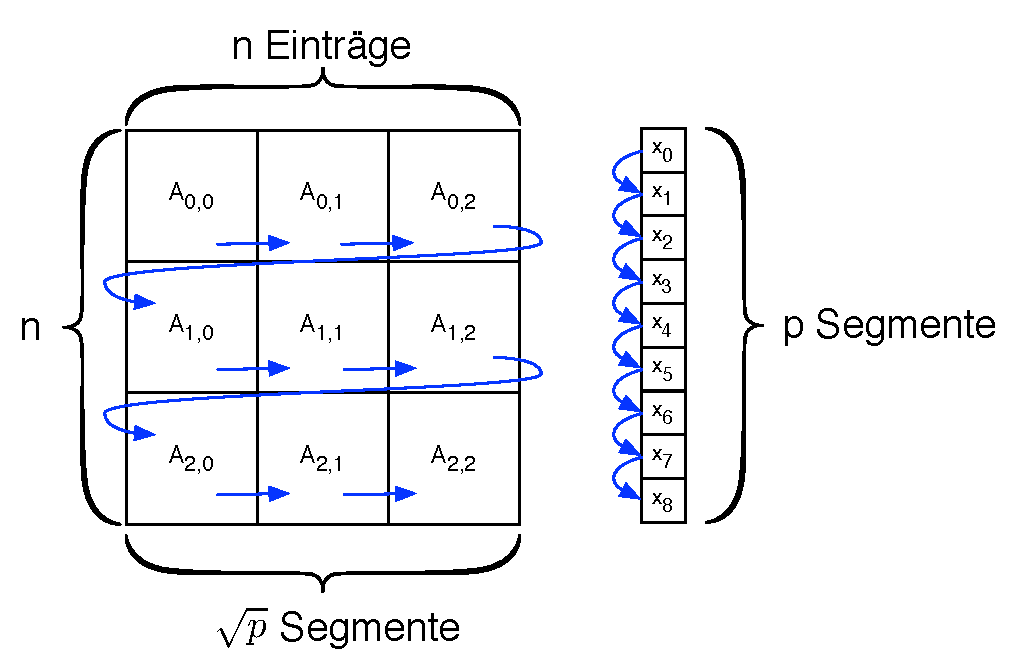
\includegraphics{pics/2d-decomposition.pdf}
	\caption{Der hier gezeigte quadratische Fall ist ein Spezialfall. n ist die Anzahl der Knoten, p die Anzahl der Places. In diesem Beispiel gibt es 9 Places. Dadurch, dass die Anzahl der Places eine Quadratzahl ist, ergibt sich horizontal und vertikal die selbe Zerlegung. Der Place mit der Nummer 0 speichert $A_{0,0}$ und $x_0$. Die blauen Pfeile zeigen, in welcher Reihenfolge die Daten auf die nachfolgenden Places aufgeteilt werden. Auf dem zweiten Place liegen demnach $A_{0,1}$ und $X_1$.}
\end{figure}

Auch bei der 2D Partitionierung müssen Vektoren auf die einzelnen Prozesse aufgeteilt werden. Angenommen die Adjazenzmatrix sei horizontal in h und vertikal in v Abschnitte unterteilt, außerdem sei n (Anzahl an Kanten) restlos durch p (Anzahl an Places) teilbar. Es gilt $h*v=p$. Die Menge der Places, die in der ersten Zeile der Unterteilung sind, besitzt dann den Abschnitt $ \left[1,n\right] * \left[1,\frac{n}{h}\right]$ der Adjazenzmatrix. Jedes Teilstück eines Vektors, den ein Place besitzt, ist  $l = \frac{1}{v} * \frac{n}{h} = \frac{n}{p}$ groß. Dadurch ist sichergestellt, dass das Teilstück eines Vektors, das der ersten Reihe gemeinsam gehört($\left[1,\frac{n}{p}\right] \cup \left[\frac{n}{p}+1,\frac{2n}{p}\right] \cup \dots \cup \left[\frac{(v-1)n}{p}+1,\frac{vn}{p}=\frac{n}{h}\right] $), dem horizontalen Teilstück $\left[1,\frac{n}{h}\right]$ des Matrixabschnittes entspricht, das genau dieser Reihe gehört.


Bei der zweidimensionalen Unterteilung wird der Breitensuch-Algorithmus als Folge von Matrix-Vektor-Operationen betrachtet, die dann einzeln parallelisiert werden. Angenommen der Algorithmus läuft auf nur einem Core, dann kann die Kommunikation und die Synchronisation eingespart werden. Der Pseudocode \ref{alg:2d_serial} beschreibt für diesen Fall die Essenz des Algorithmus. Der Algorithmus führt Iterationen aus, bis $x_k$ nur noch Nullen enthält: 
$$
x_{k+1} = \underbrace{ (A^T * x_k) }_{ \begin{tabular}{c} =1 an Stelle p \\ wenn Knoten p \\ von einem Knoten aus \\ $x_k$ erreichbar ist \end{tabular}} * \underbrace{\neg\sum_{i=1}^k x_i}_{\begin{tabular}{c} =1 an Stelle p, wenn \\ p noch unerreicht\end{tabular}}
$$ 
Das Produkt aus den beiden Vektoren entspricht der komponentenweisen Konjunktion der booleschen Werte. Die Matrixmultiplikation alleine reicht nicht aus, da Knoten sonst doppelt als erreicht markiert würden und somit eine falsche, zu große Distanz ausgegeben werden könnte. Es ist zu beachten, dass im Pseudocode die BFS-Distanz nicht gespeichert wird. Die BFS-Distanz kann aber leicht über die Nummer der Iteration herausgefunden und gesetzt werden. 

\begin{algorithm}[ht]
	\caption{BFS auf einem Place}
	\label{alg:2d_serial}
	\begin{algorithmic}[1]
		\State $f(s) \gets true$
		\State $t \gets 0^n$ // Nullvektor
		\While{$f \neq 0^n$}
			\State $x \gets A^T * f$
			\State $f \gets x * \neg t$
			\State $t \gets t + f$
		\EndWhile
	\end{algorithmic}
\end{algorithm}

Um den Code von Algorithmus \ref{alg:2d_serial} auf mehrere Places zu parallelisieren, werden die einzelnen Schritte betrachtet und die Daten entsprechend ausgetauscht. Die Zeilen 5 und 6 sind einfache eine komponentenweise Operationen und können daher lokal auf jedem Place stattfinden. In Zeile 4 wird die Matrix in der transponierten Form verwendet. Da der Algorithmus nie die nicht transponierte Form der Matrix nutzt, wird in Zukunft mit A die bereits transponierte Matrix bezeichnet. Um Zeile 4 zu parallelisieren ist einiger Aufwand notwendig. Um x[k] zu berechnen, muss sowohl die gesamte k-te Zeile aus A, als auch der gesamte Vektor f bekannt sein. Jeder Place besitzt aber nur einen Teil beider Datenstrukturen.



 Der Algorithmus wird dazu wieder in Phasen zerteilt, die in \ref{alg:2d_parallel} zu sehen sind.

 \begin{algorithm}[h]
	\caption{1D-partitionierte Breitensuche}
	\label{alg:2d_parallel}
	\begin{algorithmic}[1]
		\State {Startknoten: s, Kantenanzahl: n, Anzahl Places: p}
		\State bfsDistance : DistArray of size n \Comment{Mit $\infty$ initialisiert, 0 an Stelle s}
		\For{each place, do async on place}
			\State // Place an Position i,j im Grid
			\While{$f \neq 0$}
				\State{//Phase 1: Transpose f}
				\For{$ \mathit{node} \in \text{local part of f}$} 
					\State $j \gets \mathit{node} / \mathit{colsize} $
					\State put node in sendbuffer for column j
				\EndFor
				\State{//Phase 2: Kommunikation}
				\State{$\mathit{fTransposed} \gets \sum_{\textnormal{places in row j}}\mathit{sendbuffer}$}
				\State{$barriere$}

				\State{//Phase 3: Lokale Matrixmultiplikation}
				\For{$i=rowFrom \to rowTo$}
					\State $t[i] \gets A\big|_{i-th\;row} \cdot \mathit{fTransposed}$
				\EndFor

				\State{//Phase 4: Ergebnisse der Reihe zusammenführen}
				\For{$node \in t$}
					\State{Send node to owners \textit{t}-vector}
				\EndFor

				\State{$barriere$}
				\State{//Phase 5: Lokale updates durchführen}
				\State $f \gets t * (d==\infty)$
				\State Set d[i] = iteration number, where f[i]=true
			\EndWhile
		\EndFor
	\end{algorithmic}
\end{algorithm}
Für die folgenden Erläuterungen wird angenommen, dass es n Knoten gibt und die Adjazenzmatrix ($n \times n$) auf $g^2$ Places aufgeteilt ist, also in der Vertikalen und der Horizontalen je g Unterteilungen stattfanden. Der Place p besitze den Ausschnitt der Matrix $\left[x_{von}, x_{bis} \right] \times \left[y_{von}, y_{bis} \right]$. Dieser Ausschnitt sei der i-ten Reihe von oben und der j-te Spalte von links. 


\subsection{Phase 1: Transponieren des Vektors f} % (fold)
\label{sub:transponieren_des_vektors_f}
Es soll berechnet werden, ob Knoten k im nächsten Iterationsschritt erreicht werden kann. Dazu sei $k \in \left[y_{von}, y_{bis} \right]$. Daraus folgt, dass Place P einen Teil der Adjazenzmatix besitzt, der nötig ist, um festzustellen, ob k erreicht werden kann. Place p weiß allerdings nur, ob k von einem Knoten zwischen $x_{von}$ und $x_{bis}$ erreichbar ist. Um für diese Iteration ein Ergebnis zu berechnen, braucht er also die Information, welche dieser Knoten im Intervall $\left[x_{von}, x_{bis} \right]$ aktuell aktive Knoten sind. Diese Information ist aber aufgeteilt auf alle Places in der j-ten Reihe der Unterteilung. Für die Berechnung benötigt aber jeder der Places in der j-ten Spalte (also unter anderem Place p) genau diese Information. Deswegen wird die erste Phase als Transponieren bezeichnet. Der Algorithmus iteriert auf jedem Place über alle aktiven Knoten und berechnet, welche Spalte der Dekomposition der Matrix wissen muss, dass dieser Knoten aktiv ist. Die Formel kann beispielsweise so aussehen: $$\mathit{Spaltennummer}= \lfloor\frac{\mathit{Knotennummer}}{\mathit{Spaltenbreite}}\rfloor$$
% subsection transponieren_des_vektors_f (end)

\subsection{Phase 2: Kommunikation} % (fold)
\label{ssub:kommunikation}
Nachdem die Knoten sortiert sind, werden sie jeweils nebenläufig an den berechneten Empfänger geschickt. In der Implementierung zu dieser Arbeit steht dazu auf jedem Empfänger eine Empfangspuffer bereit. Die Verwendung eines einzelnen Empfangspuffers bedeutet, dass sich alle Sender synchronisieren müssen. Der Aufwand ist aber vernachlässigbar, verglichen mit dem Aufwand der Kommunikation. In einer optimierten Variante könnte auf jedem Place für jeden Sender ein eigener Empfangspuffer verfügbar sein, wodurch die Synchronisation wegfallen würde.
% subsection kommunikation (end)

\subsection{Phase 3: Lokale Matrixmultiplikation} % (fold)
\label{ssub:lokale_matrixmultiplikation}
Bevor dieser Schritt stattfindet, muss sichergestellt werden, dass der vorherige Schritt vollständig abgeschlossen ist. Dazu wird eine globale Barriere über alle Places verwendet. Die Matrixdatenstruktur sieht so aus, dass ein Place zu jedem Knoten in $\left[x_{von}, x_{bis} \right]$ eine Liste aller Knoten hält, die von diesem Knoten aus erreichbar sind. Es wird über alle aktiven Knoten iteriert und die Listen der erreichbaren Knoten aller aktiven Knoten aneinander gehängt. Diese Liste enthält Knoten, die in der nächsten Iteration aktiv sind, falls sie nicht schon aktiv waren. Es ist zu beachten, dass jeder Knoten in dieser Liste in dem Intervall $\left[y_{von}, y_{bis} \right]$ liegt und dass jeder Place, der ebenfalls in der i-ten Reihe ist, ein Liste von aktiven Knoten hält, die in genau demselben Intervall sind. Nur eine Reihe gemeinsam weiß exakt, welche Knoten aktiv sein werden und welche nicht.
% subsection lokale_matrixmultiplikation (end)

\subsection{Phase 4: Ergebnisse der Reihe zusammenführen} % (fold)
\label{ssub:ergebnisse_der_reihe_zusammenf_hren}
Nach dem vorherigen Schritt weiß jeder Place von einigen Knoten, dass dieser erreicht wurden. Je eine Reihe gemeinsam hat die Information, welcher von den $n/h$ Knoten, die ihnen gemeinsam gehören, erreicht wurden. Wie oben bei der Vektordekomposition zu sehen, ist jeder Knoten genau einem Place zugeordnet. Die folgende Kommunikation passiert nur zwischen Places einer Reihe, da der Abschnitt des Distanzvektors, der dieser Reihe gemeinsam gehört, genau dem Abschnitt $\left[y_{von}, y_{bis} \right]$ entspricht. Das bedeutet, dass alle Knoten, die in einer Reihe der Dekomposition stehen, untereinander austauschen müssen, welche Knoten erreicht wurde. Die Place-Nummer des Besitzers eines Knotens ist $\mathit{Placenummer}=\lfloor\frac{\mathit{Knotennummer}}{\mathit{Anzahl Places}}\rfloor$. Jeder sendet an den Besitzer des Knotens, falls dieser Knoten aktiv ist, die Knotennummer. Wenn niemand dem Besitzer eines Knotens sendet, dass dieser erreicht wurde, ist der Knoten nicht erreicht worden. Es muss auf alle Sendevorgänge gewartet werden, bevor weitere Berechnungen stattfinden können. Deswegen ist nach dieser Phase eine globale Barriere von Nöten.
% subsection ergebnisse_der_reihe_zusammenf_hren (end)

\subsection{Phase 5: Lokale Aktualisierungen durchführen} % (fold)
\label{ssub:lokale_updates_durchf_hren}
Die letzte Phase entspricht der Aktualisierung der BFS-Distanzen der konventionellen Breitensuche. Es liegt eine Liste der in dieser Iteration erreichten Knoten vor. Zu jedem Knoten ist bekannt, ob er bereits erreicht wurde oder nicht. Falls nicht, wird die BFS-Distanz auf die Nummer der aktuellen Iteration gesetzt.
% subsection lokale_updates_durchf_hren (end)
% section 2d_partitionierung (end)

\section{Allreduce} % (fold)
\label{sub:allreduce}
Ein Detail wichtiges Detail, dass bisher noch keine Erwähnung fand, findet sich sowohl in Algorithmus \ref{alg:1d_bfs_abstract} als auch in Algorithmus \ref{alg:2d_parallel} in Zeile 5. Beide Zeilen bedeuten: \textit{solange es mindestens einen aktiven Knoten gibt, iteriere...} Es gibt genau dann noch aktive Knoten, wenn mindestens ein Place mindestens einen aktiven Knoten hat. Es dürfen aber alle Prozesse auf allen Places erst dann aufhören zu iterieren, wenn auf keinem Place mehr ein aktiver Knoten vorhanden ist. In boolesches Logik ausgedrückt, muss jeder Prozess der Allgemeinheit mitteilen, ob er noch aktive Knoten hat. Diese Information muss mittels ODER verknüpft werden. Das Ergebnis der Verkñupfung muss allen Prozessen mitgeteilt werden. Diesen Vorgang nennt man an MPI angelehnt Allreduce. Es wurde die Implementierung aus der der X10 Standard Library benutzt. Falls X10 zum Beispiel über MPI kommuniziert, ist es unter Umständen wesentlich schneller, die Allreduce Operation aus einer MPI Hardware zu nutzen, als die selbe Funktionalität nachzuprogrammieren.  
% section allreduce (end)

\section{Optimierungen} % (fold)
\label{sec:optimierungen}
Auch bei der Dekomposition in zwei Dimensionen gibt es zu beachten, dass die Listen, die in Phase 3 erstellt und in Phase 4 versendet werden, Duplikate enthalten können. Um so dichter ein Graph ist, um so wichtiger ist es, diese Listen frei von Duplikaten zu machen. Siehe dazu Abschnitt \ref{sub:duplikate_in_sendepuffern}. Ohne weitere Abwandlungen kann auch die Optimierung \ref{ssub:zusammenlegung_der_ersten_und_letzten_phase} angewandt werden. Je nach gewählter Datenstruktur können auch die Adjazenzlisten wie in \ref{ssub:adjazenslisten_löschen} gelöscht werden, was bei der Implementierung zu dieser Arbeit gemacht wurde. 
% section optimierungen (end)
% chapter paralleler_algorithmus (end)
%!TEX root = thesis.tex

\chapter{Breitensuche im invasiven Kontext} % (fold)
\label{cha:breitensuche_im_invasiven_kontext}
In diesem Kapitel wird beschrieben, wie die Breitensuche unter Verwendung des Frameworks InvasIC implementiert wurde. Aus Zeitgründen konnte in dieser Arbeit nur ein Ansatz herausgearbeitet werden, der noch nicht alle Möglichkeiten des invasiven Rechnens nutzt. Deswegen ist womöglich an einigen Stellen im Algorithmus nicht sofort ersichtlich, weswegen bestimmte Lösungsansätze gewählt wurden. Das liegt daran, dass die Struktur der Implementierungen so gewählt wurde, dass zukünftige Ideen leicht umsetzbar sind.

\section{Der Algorithmus} % (fold)
\label{sec:der_algorithmus}

\subsection{Unterschiede zum nicht invasiven Fall} % (fold)
\label{sub:unterschiede_zum_nicht_invasiven_fall}
Zunächst seien in diesem Kapitel einige Unterschiede in den Anforderungen und der Problemstellung erläutert. Die Beschreibung der jeweiligen Lösungen finden sich in dann in Kapitel \ref{sub:ablauf_des_algorithmus}.

\subsubsection{Asymmetrie der Rechenleistung} % (fold)
\label{ssub:asymmetrie_der_rechenleistung}
Im invasiven Rechnen gibt es das Konzept des Processing Elements (abgekürzt PE). Ein PE ist die abstrakte Repräsentation eines Rechenkerns, auf dem ein Thread ausgeführt werden kann. Jedes PE repräsentiert genau eine Recheneinheit in der Hardware die in einem bestimmten Bereich mit gemeinsamen Speicher liegt. Dieser Bereich mit gemeinsamen Speicher wird durch X10 mittels Places abstrahiert. Es kann zum Beispiel ein Prozessor mit 8 Cores vorliegen. Im InvasIC-System existieren dann 8 PEs, die alle auf dem selben Place liegen. Synchronisation und Kommunikation zwischen zwei Activities auf dem selben Place geht wesentlich schneller, was sowohl Bandbreite als auch einmalige Startzeit der Kommunikation betrifft, als wenn die Activities auf unterschiedlichen Places liegen. 

Die Breitensuche wie in Kapitel \ref{sec:1d_partitionierung} behandelt das Problem, indem er auf jedem Place gleich viele Daten und damit gleichviel Rechenarbeit legt. Es wird auf jedem Place zunächst genau eine Activity gestartet, die dann zum Beispiel auf Schleifenebene Nebenläufigkeit erzeugt. Es gibt quasi zwei klare Hierarchiestufen der Parallelität. Dieser Ansatz geht davon aus, dass alle Places gleich schnell rechnen.

Im invasiven Fall fragt das Programm bei dem Agenten nach Rechenleistung und bekommt daraufhin eine gewisse Menge an PEs als Antwort zurück. Selbst wenn durch Constraints festgelegt würde, dass die PEs gleichmäßig auf Places verteilt sein sollen, kann der Agent das in Abhängigkeit der aktuellen Situation des Gesamtsystems nicht garantieren. Deswegen kann sich das Programm nicht darauf verlassen. Das Programm findet sich also in der Situation, dass es beispielsweise drei PEs, eine auf Place 0 und zwei auf Place 3 hat. Die erste Konsequenz muss sein, dass auf Place 3 doppelt so viele Daten wie auf Place 0 liegen. Im Falle der Breitensuche werden Place 3 also doppelt so viele Knoten gehören wie Place 0. Wird nun ein infect auf die drei PEs aufgerufen, werden korrekterweise drei Activities gestartet, die alle denselben Code ausführen. Allerdings stehen die zwei Activities, die auf dem selben Place laufen, in einem anderen Verhältnis zueinander, als zwei Activities, die auf verschiedenen Places laufen. Die Activities haben für die folgenden Erläuterungen die Nummern 0,1 und 2, wobei Activity 0 auf Place 0 und entsprechen 1 und 2 auf Place 3 liegen.
% TODO: Andreas fragen, ob das wirklich nicht garantiert werden kann (Zeile hier drüber)
\begin{itemize}
	\item Will Activity 0 Daten an 1 und 2 schicken, so ist es effizienter diese in einem Kommunikationsvorgang zusammenzufassen, als das IPC-System zweimal zu starten
	\item Ebenso sollten Activity 1 und 2 gemeinsam ihre Daten an Activity 0 schicken.
\end{itemize}
% subsubsection asymmetrie_der_rechenleistung (end)
Eine Activity muss also den gesamten Kontext kennen und wissen, ob und in welchem Fall sie sich mit anderen Activities auf dem selben Place zusammen tun muss.

\subsubsection{Dynamische Ressourcenverwaltung und Verteilung der Daten} % (fold)
\label{ssub:dynamische_ressourcenverwaltung}
Hier ist prinzipiell ein Designentscheidung zu treffen, da sich zumindest bei der Breitensuche nur schwer folgende Ziele vereinbaren lassen:
\begin{itemize}
	\item Dynamisches invade und retreat je nach benötigter Rechenleistung.
	\item Daten so verteilen, dass die Rechenleistung ideal ausgenutzt wird.
\end{itemize}
\underline{Erklärung:} Die Situation sei wie in \ref{ssub:asymmetrie_der_rechenleistung}, eine PE auf Place 0, zwei PEs auf Place 3. Es sei bereits eine Iteration der Breitensuche abgeschlossen. Nun ist bekannt, wie viele der Knoten, die auf Place 0 liegen, aktiv sind und wieviel Knoten, die auf Place 3 liegen, aktiv sind. Die Situation sei so, dass beide ungefähr gleich viele Knoten in der nächsten Iteration zu bearbeiten haben, obwohl auf Place 3 ja die doppelte Menge an Knoten liegt. Die doppelte Rechenleistung auf Place 3 ist damit in der nächsten Iteration nicht zu gebrauchen, da die beiden Activities auf Place 3 nach der abgeschlossenen Iteration auf Place 0 warten müssten, der für die selbe Iteration ungefähr doppelt so lange benötigen wird. Eine ressourcengewahres System würde also eine der beiden PEs auf Place 3 abgeben. Jetzt steht auf den beiden Places gleichviel Rechenleistung zu Verfügung. Durchschnittlich ist die Liste der aktiven Knoten auf Place 3 aber doppelt so lang wie die Liste auf Place 0. Die Anwendung kann nun in einer späteren Iteration versuchen, wieder eine PE auf Place 3 zu bekommen. Allerdings kann diese bereits von einer anderen Anwendung besetzt sein. Zudem entspricht es nicht exakt dem Paradigma des invasiven Rechnens, dem Agenten mitteilen zu müssen, welche PE genau gewünscht ist.

Die naheliegende Antwort auf dieses Problem ist die Umverteilung der Daten, so dass gleich viele Daten auf Place 0 und 3 liegen, zumindest bis die gewünschte PE wieder verfügbar ist. Dieser Ansatz wurde im Rahmen dieser Arbeit nicht betrachtet, da er zum einen sehr aufwendig zu implementieren ist und zum anderen zu erwarten ist, dass die Performance sehr schlecht ist. Es müssten große Datenmengen (Adjazenzlisten, Distanzarrays) verschickt werden, größere Arrays alloziert werden, usw.

Zusammenfassend kann man sagen, dass ein Algorithmus, der auf partitionierten Daten (ein Graph bei BFS) arbeitet, nur sehr schwierig gleichzeitig temporär ungenutzte Ressourcen abgeben und trotzdem noch maximal effizient arbeiten kann. In dieser Arbeit entspricht zwar jede BFS-Iteration einem \textit{invade}, allerdings werden zwischen den Iterationen keine Ressourcen abgegeben oder angefordert.
% subsubsection dynamische_ressourcenverwaltung (end)

\subsubsection{Nicht fortlaufende Indizes} % (fold)
\label{ssub:nicht_fortlaufende_indizes}
Trotz Verwendung des InvaIC Frameworks, soll die X10 API weiter genutzt werden können. Die X10-Funktionalitäten rund um Distributions, und DistArrays arbeitet auf der Basis von Places und deren Nummerierung. Aus diesem Grund kann man im invasiven Fall nicht komplett von der Vorstellung von Places weggehen, sondern muss im Auge behalten, auf welchem Place welche Daten liegen. Im reinen X10 sind die Places immer von 0 bis p-1 (bei p Places) durchnummeriert. Das macht die Nummer eines Places zu einem sehr praktischen Ausgangspunkt, um mit Indizes zu rechnen. Es kann zum Beispiel ein DistArray der Größe p erstellt werden, wenn auf jedem Place genau ein Datum liegen soll und jeder Place kann mit seinem eigenen Index auf seine eigenen Daten zugreifen.

Im invasiven Fall werden vom Agent zunächst nur ProcessingElements bereitgestellt. Auf welchem Place diese liegen, ist für den Klienten völlig unvorhersehbar und unbeeinflussbar. Dadurch ist keine natürliche Nummerierung der Places vorhanden. Es lässt sich nicht vermeiden, etwas Speicherplatz und Rechenleistung zu benutzen, um dieses Problem zu lösen. Der unten stehende Vergleich des Codes zum Feststellen, welcher der besitzende Place von Knoten k ist, verdeutlicht das Problem. $p$ ist die Anzahl an Places, \textit{placesList} eine Liste aller Places und \textit{mapNodeToPlaceIndex} ein Funktion. Damit diese Funktion funktioniert, muss vorher schon eine Datenstruktur mit dem vollständigen wissen über alle PEs initialisiert worden sein.
\begin{algorithm}
	\caption{Durchnummerierter Fall, wie in Kapitel \ref{sec:1d_partitionierung}}
	\label{alg:owner_consecutive}
	\begin{algorithmic}[1]
		\State \textbf{val} owner = k / p
	\end{algorithmic}
\end{algorithm}

\begin{algorithm}
	\caption{Nicht durchnummerierter Fall, wie in diesem Kapitel}
	\label{alg:owner_random}
	\begin{algorithmic}[1]
		\State \textbf{val} ownerId = mapNodeToPlaceIndex(k) // Position des owners in der placesList
		\State \textbf{val} owner   = placesList[ownerId]
	\end{algorithmic}
\end{algorithm}
% subsubsection nicht_fortlaufende_indizes (end)

% subsection unterschiede_zum_nicht_invasiven_fall (end)
\subsection{Ablauf des Algorithmus} % (fold)
\label{sub:ablauf_des_algorithmus}
Aus Zeitmangel wurde im Rahmen dieser Arbeit die Breitensuche im invasiven Fall nur mittels der 1D-Dekomposition implementiert. Grundsätzlich ist der selbe Algorithmus wie in Kapitel \ref{sec:1d_partitionierung} beschrieben implementiert. In diesem Kapitel werden deswegen in erster Linie die gewählten Lösungsansätze zu den Problem aus Kapitel \ref{sec:der_algorithmus} beschrieben.
\begin{figure}[ht]
	\centering
	\label{img:invasive-flow}
	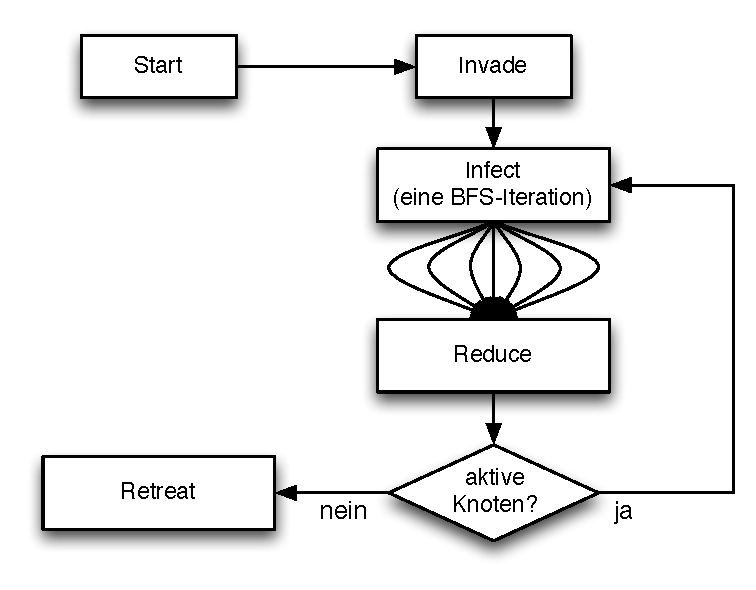
\includegraphics{pics/invasive-flow.pdf}
	\caption{Grundsätzlicher Ablauf der Breitensuche. Zu beachten ist, dass zwischen den einzelnen Iterationen kein \textit{retreat} und kein invade stattfindet.}
\end{figure}

\subsubsection{Dekomposition und Datenhaltung} % (fold)
\label{ssub:dekomposition_und_datenhaltung}

Sobald der Algorithmus nach dem Start den Graph vollständig eingelesen hat und die Antwort des \textit{invade} bekommen hat (eine Liste von PEs), beginnt er damit, sich die benötigten Datenstrukturen aufzubauen.
\begin{itemize}
	\item ProcessingElements nach Placenummer sortieren. Liste alle involvierten Places in eben dieser Reihenfolge aufstellen und zu jedem Place die Anzahl an verfügbaren PEs in ein Array schreiben. An der Stelle 0 in diesem Array steht also, wie viele PEs auf dem Place zur Verfügung stehen, der in der Placeliste an erster Stelle (Index 0) steht.
	\item Die Menge an Knoten wird so unterteilt, dass jede PE ein gleichgroßen Teil bekommt. Wichtig ist, dass alle PEs, die auf dem selben Place liegen, benachbarte Intervalle der Knotenliste bekommen. Es wird entsprechend Platz für die Adjazenzlisten auf den Places reserviert. Alle Knoten, die zu einem Place gehören, gehören allen dortigen PEs gemeinsam. Um aufzulösen, welchem Place ein Knoten gehört, wird ein Array berechnet, dass für jede PE (in der Reihenfolge der Liste aus dem ersten Punkt) enthält auf welchem Place sie liegt. Um den Besitzer von Knoten k zu finden, muss so zur Laufzeit nur noch k durch die Anzahl an PEs geteilt werden. Das Ergebnis ist die Stelle der Placeliste, an der der besitzende Place steht.
	\item Das Selbe muss für das DistArray passieren, dass die BFS-Distanzen halten soll.
	\item Es wird pro Place für jeden anderen Place ein Empfangspuffer erstellt. Diese Empfangspuffer befinden sich in einem DistArray mit einer UniqueDist, das bedeutet, dass auf jedem Place genau ein Datum(=Array aus Puffern) liegt.
	\item Es wird pro Place eine Liste für aktive Knoten erstellt.
\end{itemize}

% subsubsection dekomposition_und_datenhaltung (end)
\subsubsection{Zweistufiges Infect und Indizierung} % (fold)
\label{ssub:zweistufiges_infect}
Der Algorithmus verwendet die \textit{Clock}-Funktionalität von X10. Eine Clock entspricht einer Barriere, die alle Aktivitäten bei Erreichen so lange blockiert, bis alle registrierten Aktivitäten die Barriere erreicht haben. Es wird sowohl für alle Aktivitäten (es gibt eine Aktivität pro PE) global eine Clock benötigt, als auch lokal zwischen je allen Aktivitäten, die auf dem selben Place liegen. Um diese Clocks zu erstellen, ist es nötig den Infect-Aufruf manuell zweistufig zu implementieren. Zunächst wird die globale Clock erstellt, dann wird eine Aktivität pro involviertem Place gestartet, die sich aber nicht in der Clock registrieren. Anschließend wird von der einen Aktivität auf jedem Place eine weitere Clock erstellt und pro PE, die auf diesem Place zur Verfügung steht eine Aktivität gestartet. Diese Aktivität registriert sich jetzt in beiden oben erstellten Clocks und beginnt mit der BFS.

Ein weiterer Vorteil des zweistufigen Infects ist es, dass sehr einfach jeder Aktivität ein globaler Index und ein lokaler Index gegeben werden kann. Der lokale Index ist die Nummer einer Aktivität auf einem Place. Vor allem der lokale Index wird im Weiteren sehr nützlich sein.
% subsubsection zweistufiges_infect (end)

\subsubsection{Lokale Parallelität} % (fold)
\label{ssub:lokale_parallelit_t}
Wie die Kollaboration zwischen den einzelnen Places aussieht wurde bereits in Kapitel \ref{sec:1d_partitionierung} beschrieben. Ein Place als ganzes Verhält sich im invasiven Fall exakt gleich. Allerdings gibt es keine \enquote{Masteraktivity} pro Place, die Jobs verteilen kann und für die Synchronisation sorgt. Stattdessen werden mehrere gleichberechtigte Activities gestartet, die trotzdem auf den selben Daten arbeiten sollen. In diesem Abschnitt wird beschrieben, wie diese Zusammenarbeit gelöst wurde. Dazu werden die Phasen aus Kapitel \ref{sec:1d_partitionierung} aufgegriffen. Eine genaue Beschreibung der einzelnen Phasen findet sich auch dort und wird hier nicht wiederholt. Wichtig ist, dass jede Activity die Information hat, die wievielte von wie vielen sie auf diesem Place ist.

\subsection{Phase 1: Adjazente Knoten sortieren} % (fold)
\label{sub:phase_1_invasive}
Die Liste der aktiven Knoten ist einmal pro Place vorhanden. Sie ist als Arrayliste implementiert und ermöglicht somit schnellen Zugriff auf beliebige Elemente. In Phase 1 wird die Liste in gleichgroße Stücke aufgeteilt, so dass jede Activity auf dem Place ein Stück bekommt. Es steht pro Zielplace aber nur ein Sendpuffer zur Verfügung, in welchen alle ACtivities konkurrierend schreiben. Deswegen muss sichergestellt werden, dass der Zugriff auf jeden Buffer atomar passiert. Nach dieser Phase ist lediglich eine lokale Barriere nötig um sicherzustellen, dass alle Sendepuffer korrekt und vollständig geschrieben wurden. 
% subsection phase_1 (end)

\subsection{Phase 2: Kommunikation} % (fold)
\label{sub:parallel_phase_2_invasive}
In Phase 2 werden die Sendepuffer gesendet. Eine Aktivität ist für einen Sendepuffer genau dann zuständig, wenn die ID des Ziels modulo der Anzahl an Activities auf diesem Place der lokalen ID dieser Aktivität entspricht. Ansonsten ist hier nichts anzupassen. Nach dem Senden wird eine globale Barriere benötigt, damit alle Empfangspuffer korrekt geschrieben wurden, bevor diese ausgewertet werden.
% subsection phase_2 (end)

\subsection{Phase 3: BFS-Distanz aktualisieren} % (fold)
\label{sub:phase_3_invasive}
Wie in Phase 2 liest eine Activity genau dann einen Empfangspuffer, wenn die ID des Senders modulo Anzahl an Activities auf diesem Place die lokale ID der Activity ergibt. Diese Aufteilung der Arbeit entspricht nicht unbedingt einer gleichmäßigen Aufteilung der Arbeit, geht aber fast ohne Synchronisation. Einzig die Liste der aktiven Knoten für die nächste Iteration muss atomar geschrieben werden.
% subsection phase_3 (end)

% subsubsection lokale_parallelit_t (end)
\subsubsection{Allreduce} % (fold)
\label{ssub:allreduce_invasive}
Das Allreduce ist im invasiven Fall insofern nicht mehr nötig, als dass es keine All-to-All Operation mehr ist. Es wird ohnehin nach jeder BFS-Iteration zunächst die Berechnung gestoppt und nur falls eine weitere Iteration nötig ist erneut ein \textit{infect} aufgerufen. Das Ergebnis der aktuellen Iteration schreiben alle Activities in ein Array, das Anfangs erstellt wird und dass eine Zelle für jede Activity bereithält. Um das Array zu adressieren, wird jeder Activity eine GlobalRef übergeben. Die Master-Activity reduziert dieses Array dann lokal um festzustellen, ob der Algorithmus fertig ist. Falls nicht, wird eine weitere Iteration gestartet.
% subsubsection allreduce (end)
% subsection ablauf_des_algorithmus (end)
% section der_algorithmus (end)	


% chapter breitensuche_im_invasiven_kontext (end)
%!TEX root = thesis.tex

\chapter{Methoden} % (fold)
\label{cha:methoden}

\section{Graphen} % (fold)
\label{sec:graphen}
Die Breitensuche auf einem 1.2GB Beispielgraph läuft, je nach Algorithmus, in knapp einer Sekunde durch (Anhang \ref{Anhang-Messwerte-Dichte}). Wenn ein Algorithmus nur sehr kurz läuft, machen konstante Laufzeitschwankungen prozentual einen größeren Anteil aus. Wenn also beispielsweise ein Algorithmus durch das Betriebssystem, das gerade etwas andere machen muss, für 10ms unterbrochen wird, verfälscht das eine Messung die nur 50 ms läuft gravierender, als eine Messung, die mehrere Sekunden läuft. Deswegen wurde versucht, größtmögliche Beispielgraphen zu generieren. Für diese Arbeit wurden Graphen in der Größenordnung von 100 000 Knoten generiert. Diese wiederum relativ kleine Ausdehnung wurde gewählt, da der Testmodus unter anderem beinhaltet, dass bei gleichbleibender Knotenanzahl die Dichte des Graphen variiert. Sehr dicht besiedelte Graphen mit 100 000 Knoten passen gerade noch in den Arbeitsspeicher. Würden noch größere Graphen verwendet, müsste entweder die Dichte des Graphen beschränkt werden oder das Betriebssysteme müsste Speicherseiten auslagern. Da die Zeit für die Auslagerung mit in die Laufzeitmessung eingehen würde, ist zu erwarten, dass der Algorithmus dadurch deutlich langsam wäre, als bei Probleminstanzen, die in den Hauptspeicher passen. Die einzige Schlussfolgerung aus so einer Testreihe wäre, dass externe Algorithmen langsamer sind, als interne. 

Die asymptotische Laufzeit der Breitensuche ist O(n + m) ist \cite{SWB-283374373}. Das führt zu der Vermutung, dass bei gleicher (absoluter) Kantenzahl und erhöhter Knotenzahl, die Laufzeit nicht wesentlich länger ist. Ein Beispiel: BFS auf einem Graph mit 1 000 000 Knoten und durchschnittlichem Knotengrad von 100 (ergibt 100 Mio Kanten) sollte kaum länger dauern, als die BFS auf einem Graph mit 100 000 Knoten und durchschnittlichem Knotengrad von 1000 (ergibt ebenso 100 Mio Kanten). Diese Annahme ist für den parallelen Fall falsch, da die zu versendenden Datenmengen erheblich größer werden, wenn der Graph mehr Knoten hat.

Es wurde ein Tool namens graph-generator \cite{graph-generator:2009:Online} eingesetzt, um zufällige Graphen zu generieren. Um einen Graph zu erstellen, müssen folgende Parameter übergeben werden:
\begin{enumerate}
	\item Die Anzahl an Knoten.
	\item Der minimale Ausgangsgrad jedes Knotens.
	\item Der maximale Ausgangsgrad jedes Knotens.
	\item Der Exponent der Exponentialverteiltung.
	\item Der mittlerer Knotengrad z.
\end{enumerate}
Der Ausgangsgrad der Knoten ist folgendermaßen verteilt:
$$
P(X=k) \propto (k + offset)^{-exp}
$$
Der Offset wird dabei automatisch von dem Tool derart gewählt, dass sich ein durchschnittlicher Ausgangsgrad von z ergibt. Der Exponent der Exponentialverteilung \textit{exp} wurde vor den ersten Messungen auf 5 festgelegt und danach nicht mehr verändert. Die Zahl 5 wurde nach Tests mit verschiedenen Exponenten insofern als geeignet angesehen, als dass die Wahrscheinlichkeiten für Knoten mit sehr geringem Grad nicht zu hoch waren. Mit noch größeren Exponenten hatte der graph-generator Probleme.
% section graphen (end)

\section{Testplattform} % (fold)
\label{sec:testplattform}
Als Testplattform kann ein Apple Notebook von 2011 zum Einsatz. Es hat einen Intel Core i7-2720QM \enquote{Sandy Bridge} Prozessor, der mit 2.2Ghz getaktet wird. Es stehen 4 physikalische Kerne zur Verfügung, die jeweils Intels Hyper Threading Technologie unterstützen. Dadurch sind physikalisch 8 parallel laufende Threads möglich. Beim Vergleich von sequentiellen Algorithmen mit parallelen ist zu beachten, dass der Prozessor einen Kern auf bis zu 3.3 GHz übertakten kann, falls die anderen Kerne momentan nicht verwendet werden. Der optimal erreichbare Speedup ist demnach nicht 8.0, sondern deutlich darunter. Das Testsystem ist außerdem mit 8GB Hauptspeicher ausgestattet, der bei einem Takt von 1333Mhz arbeitet. Auf dem Testsystem wird als Betriebssystem Mac OS X 10.6.8 \enquote{Snow Leopard} und der x10 Compiler in der Version 2.2.3 verwendet.
% section testplattform (end)

\section{Modus} % (fold)
\label{sec:modus}
Um Ergebnisse aus je einer Algorithmus - Graph - Kombination zu erhalten, wird der gewählte Algorithmus drei mal auf dem gewählten Graph ausgeführt und die Zeit gemessen, die die Berechnung benötigt. Die Zeit, um den Graph in den Speicher einzulesen und die Daten auf die Places aufzuteilen, wurde nicht gemessen, da sie wenig mit dem Algorithmus oder X10 zu tun hat. Die Zeit, die benötigt wird, um das Ergebnis von den beteiligten Places zurück zum Ursprungsplace zu kopieren, wird allerdings mitgemessen.

Die X10 Laufzeitumgebung liest beim Programmstart die beiden Umgebungsvariablen X10\_NPLACES und X10\_NTHREADS, in denen steht, wie viele Places lokal auf diesem Rechner simuliert werden sollen und wie viele Threads jedem dieser Places zur Verfügung stehen sollen. Die einzelnen Places werden durch Prozesse (nicht Threads) repräsentiert, wodurch sie tatsächlich getrennte Speicherbereiche haben. Dieser Aufbau entspricht zwar nicht einem Setup, in dem jeder X10 Prozess auf einen physikalisch getrennten Computer operiert, doch auch der Kontextwechsel, der bei der Kommunikation zwischen Places auftritt, ist relativ langsam und somit eine Annäherung an realen Kommunikationsoverhead. Trotzdem sind diese Ergebnisse nicht eins zu eins auf einen Rechnerverbund zu übertragen. Das liegt zum einen daran, dass, die Kommunikation zwischen physikalisch getrennten Places nochmal erheblich teurer ist, als lokale Interprozesskommunkation, zum anderen können mit einem Rechnerverbund wesentlich größere Graphen bearbeitet werden, deren Effekte auf den Algorithmus in dieser Arbeit nicht gemessen werden.
Andererseits dürfen die Ergebnisse dieser Arbeit auch nicht mit der lokalen Parallelisierung der Breitensuche auf einem einzelnen Rechner verwechselt werden. Kommunikation mittels geteiltem Speicher ist deutlich schneller, als die hier verwendete Interprozesskommunikation. Es sei hier auch nochmal darauf hingewiesen, dass pro Prozess, also pro Place, immer nur ein Thread aktiv ist.
Um die Möglichkeit der Parallelität zu messen, wurde der Algorithmus in der 1D und der 2D Zerlegung jeweils in einer Konfiguration mit 1, 2, 4, 8 und 9 Places ausgeführt. Die Konfiguration mit 9 Places wurden hinzugenommen, da so bei der 2D Zerlegung eine symmetrische 3 mal 3 Zerlegung stattfinden kann. Es wurde vermutet, dass eine quadratische Anzahl an Places besonders günstig für diesen Algorithmus sind, obwohl 9 Places mehr sind, als Rechenkerne zur Verfügung stehen. Der Vollständigkeit halber wurde auch der 1D Algorithmus mit 9 Places durchgeführt. Um wirklich vollständige Ergebnisse zu bekommen, sollte eigentlich pro Graph die Breitensuche einmal von jedem Knoten aus gestartet werden.  Dieses Unterfangen würde den Zeitrahmen der Arbeit sprengen.

Der Modus, mit nur einem Thread pro Place und ohne die Nutzung von geteilten Speicher zwischen den einzelnen Ausführungsfäden lässt neben der Übertragbarkeit auf die invasive Hardware auch Rückschluss auf Manycore - Systeme zu. Bei diesen CPUs der Zukunft sollen viele kleine Rechenkerne auf einer CPU platziert werden. Cachekohärenz mit geteiltem Speicher und sehr vielen Kernen benötigt viel Overhead. Es werden deswegen auch Ansätze ohne geteilten Speicher verfolgt. Auch wird jeder Kern nur einen Ausführungsfaden gleichzeitig bearbeiten können. Die hier vorgeschlagenen Implementierungen sind also für solch eine Hardware interessant.
% section modus (end)

\chapter{Ergebnisse und Diskussion} % (fold)
\label{cha:ergebnisse_und_diskussion}

Die vollständigen Messergebnisse finden sich in den Anhängen \ref{Anhang-Messwerte-Dichte}, \ref{Anhang-Messwerte-Verteilung} und \ref{Anhang-Messwerte-Groesse}. Es wurden die Auswirkungen der Variation der Dichte, der Knotenzahl und der Verteilung des Graphen auf die Laufzeit gemessen, wobei jeweils die anderen Parameter fest gewählt waren. Sehr dünn besetzte und kleine Graphen waren deutlich schneller mit einer seriellen Version der Breitensuche zu lösen, als es mit jedwedem parallelen Algorithmus möglich war. Der Vergleich der seriellen Breitensuche, mit der 1D-Breitensuche mit einem Place ist durchaus auch interessant und wird in Kapitel \ref{sec:serieller_fall_vs_1d_mit_einem_place} vertieft. Der 2D-Algorithmus war in allen Testfällen der langsamste, weswegen er gesondert in Kapitel \ref{sec:die_2d_breitensuche} behandelt wird.

\section{Serieller Fall, 1D mit einem Place und 2D mit einem Place} % (fold)
\label{sec:serieller_fall_vs_1d_mit_einem_place}
Jeder Algorithmus muss pro Iteration jeden aktiven Knoten mindestens einmal in irgendeiner Weise bearbeiten. Außerdem muss jeder Algorithmus pro Iteration jeden der Knoten mindestens einmal bearbeiten, der von einem der aktiven Knoten aus erreichbar ist. Der serielle Algorithmus tut genau das und nicht mehr. In Tests wurde herausgefunden, dass eine Iteration mittels einer herkömmlichen for-Schleife mit anschließendem direkten Elementzugriff über den Index deutlich schneller ist, als eine foreach-Schleife. Der 1D-Algorithmus muss pro Iteration die Knoten in Sendepuffer einsortieren (jeden aktiven Knoten einmal bearbeiten) und verschicken, was im Fall mit nur einem Place aber eine einfache Zeigerzuweisung ist. Anschließend muss dann nochmals jeder aktive Knoten betrachtet werden, um alle erreichbaren Knoten zu erhalten. Der 1D-Algorithmus muss also zweimal über alle aktiven Knoten iterieren, zumindest in einer naiven Implementierung. Die verwendete optimierte Version legt diese beide Phasen aber zusammen. Zusätzliche Arbeit, im Gegensatz zu der seriellen Version, hat der 1D Algorithmus also nur beim Zurückkopieren des gesamten BFS-Distanz-Arrays.

Die Messergebnisse sind in Abbildung \ref{fig:Vergleich_Seriell} illustriert. Sie zeigen, dass der serielle Algorithmus für dichte Graphen langsamer ist, als der 1D Algorithmus, wenn er mit nur einem Place gestartet wird. Nur bei dünn besetzten Graphen ist die Laufzeiten des seriellen Algorithmus ein Wenig schneller, wobei die Grenze bei den Tests bei einem durchschnittlichen Knotengrad von ca. 400 lag. Die Messergebnisse zur Variation der Größe (Kapitel \ref{sub:gr_e}) zeigen ebenfalls, dass auch bei großer Knotenzahl der serielle Algorithmus der schnellste ist, solange der durchschnittliche Knotengrad nicht zu groß wird.

Wieso der serielle Algorithmus auf Listenbasis nicht der schnellste ist, wie eigentlich erwartet, ist nicht ohne weiteres zu erklären. Zufall in Verbindung mit der Garbage Collection sind in Anbetracht der Deutlichkeit der Ergebnisse auszuschließen. Eine mögliche Erklärung ist, dass der Compiler den einen Code besser optimieren konnte, als den anderen, ohne dass sofort offensichtlich ist, woran das liegt.

Wie ebenfalls aus Abbildung \ref{fig:Vergleich_Seriell} hervorgeht, ist der 2D Algorithmus deutlich langsamer als die beiden anderen. Der 2D Algorithmus hat zwei Kommunikationsphasen pro Iteration. In den beiden Phasen wir aber jeweils nur mit $\sqrt(p)$ anderen Places kommuniziert (bei p Places)\cite{Buluc:2011}, während im Fall des 1D Algorithmus jeder Place potentiell mit allen anderen kommuniziert. Im seriellen Fall ist diese zusätzliche Komplexität nicht nötig, verlangsamt aber den Ablauf.
% section serieller_fall_vs_1d_mit_einem_place (end)  

\begin{figure}
	\centering
	\label{fig:Vergleich_Seriell}
	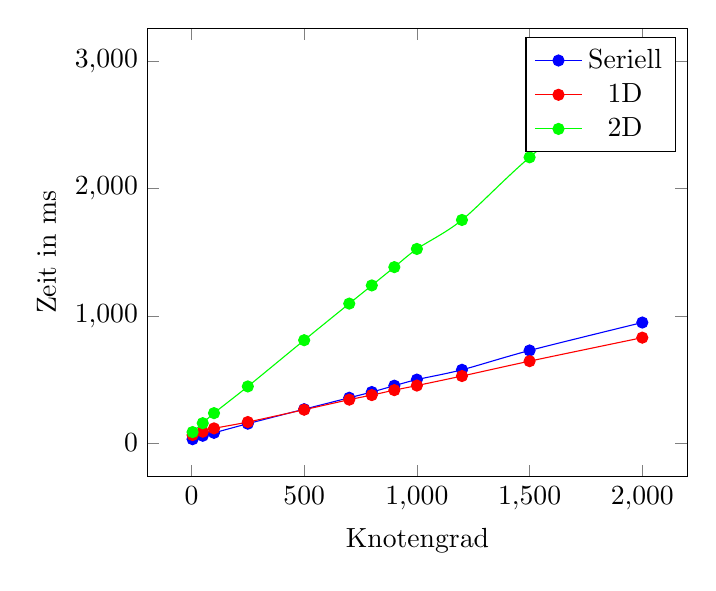
\begin{tikzpicture}
	    \begin{axis}[
	        xlabel=Knotengrad,
	        ylabel=Zeit in ms]
	    \addplot[smooth,mark=*,blue] plot coordinates {
	        (5,29)
	        (50,56)
	        (100,79)
	        (250,151)
	        (500,265)
	        (700,355)
	        (800,400)
	        (900,450)
	        (1000,498)
	        (1200,575)
	        (1500,727)
	        (2000,947)
	    };
	    \addlegendentry{Seriell}

	    \addplot[smooth,color=red,mark=*]
	        plot coordinates {
	        (5,62)
	        (50,88)
	        (100,114)
	        (250,164)
	        (500,261)
	        (700,340)
	        (800,376)
	        (900,415)
	        (1000,451)
	        (1200,526)
	        (1500,643)
	        (2000,828)
	        };
	    \addlegendentry{1D}

	    \addplot[smooth,color=green,mark=*]
	        plot coordinates {
	        (5,85)
	        (50,155)
	        (100,234)
	        (250,444)
	        (500,808)
	        (700,1096)
	        (800,1239)
	        (900,1383)
	        (1000,1526)
	        (1200,1754)
	        (1500,2247)
	        (2000, 2969)
	        };
	    \addlegendentry{2D}
	    \end{axis}
	\end{tikzpicture}
	\caption{Vergleich der Laufzeiten bei serieller Ausführung, also nur ein Place bei 1D und 2D Algorithmus, jeweils schnellste gemessene Laufzeit.}
\end{figure}

\section{Ergebnisse der Parallelisierung} % (fold)
\label{sec:ergebnisse_der_parallelisierung}
Da die Breitensuche mit dem 2D Dekomposition keine vergleichbaren Ergebnisse lieferte, wird hier nur der serielle Algorithmus mit dem 1D Algorithmus verglichen. Mehr zu der 2D Breitensuche ist in Kapitel \ref{sec:die_2d_breitensuche} niedergeschrieben. Es wurden drei Testreihen durchgeführt.
\begin{description}
	\item[Dichte] Der Knotenzahl und die Verteilung sind konstant, die Kantenanzahl variiert. \newline Die Knotenzahl ist 100 000, die Grenzen des Knotengrads sind konstant zwischen 1 und $\infty$
	\item[Verteilung] Die Knotenzahl und Kantenanzahl sind konstant, die Grenzen des Knotengrads variieren.\newline Die Knotenzahl ist 100 000, der Knotengrad 750
	\item[Größe] Der durchschnittliche Knotengrad und die Grenzen des Knotengrads sind konstant, die Knotenzahl variiert. Der durchschnittliche Knotengrad ist 100, der minimale Knotengrad 1, der maximale 500.
\end{description}
Diese Werte sind auch aus Tabelle \ref{tab:Testreihen} ersichtlich.

\begin{table}
\label{tab:Testreihen}
\begin{tabular}{p{3.7cm}|c|c|c}
  & Testreihe \enquote{Dichte} & Testreihe \enquote{Verteilung} & Testreihe \enquote{Größe} \\ \hline \hline
  Knotenzahl & konstant 100 000 & konstant 100 000 & variiert\\
  Kantengrad \o & variiert & konstant 750 & konstant 100\\
  Kantengrad Grenzen & konstant $\ge$1, $<\infty$ & variiert & konstant $\ge$1, $\le$500\\
 \end{tabular}
  \caption{Jede Testreihe besteht aus mehreren Graphen. Der Eintrag \enquote{variiert} bedeutet, dass diese Maßzahl zwischen den Graphen dieser Reihe variiert. Im Gegensatz dazu bedeutet \enquote{konstant}, dass diese Maßzahl für alle Graphen dieser Reihe gilt.}
\end{table}

\newpage
%!TEX root = thesis.tex
\subsection{Dichte} % (fold)
\label{sub:dichte}
Die hier behandelten Graphen haben 100 000 Knoten bei einem minimalen Knotengrad von 1. Nach oben ist der Knotengrad nicht beschränkt. Als Dichte wird hier das Verhältnis von Kanten zu Knoten bezeichnet. Dieses Verhältnis ist gleichzeitig der durschnittliche Knotengrad. Der Knotengrad ist auf nur 100 000 beschränkt, um sehr dichte Graphen trotzdem noch in den Hauptspeicher zu bekommen. Die vollständigen Ergebnisse der Testreihe sind unter \ref{Anhang-Messwerte-Dichte} anggehängt.

Die Messergebnisse liefern kein eindeutiges Bild. Aus Abbildung \ref{fig:max_speedup} ist leicht ersichtlich, dass eine mindeste Graphgröße vorhanden sein muss, damit es sich überhaupt lohnt, parallel an einer Instanz des BFS zu arbeiten. Dabei scheint nicht nur die Anzahl der Knoten relevant zu sein, sondern auch die Anzahl der Kanten. Auffällig ist, dass der Speedup mit steigender Dichte nicht wächst. Der maximal erreichte Speedup liegt bleibt im Bereich zwischen 1.2 und 1.3, bis auf den einen Aussetzer. Der Aussetzer ist ohne weiter Analyse des Graphen nicht zu erklären. Es ist unwahrscheinlich, dass gerade bei einer bestimmten Graphdichte die Parallelisierung dermaßen viel besser funktioniert, als bei allen anderen Graphdichten. Wahrscheinlicher ist es, dass der Zufallsgenerator einen Graph generiert hat, der wenig Kanten zwischen Knoten hat, die auf unterschiedlichen Places liegen. Es kann auch sein, dass durch Zufall die Last auf den Places bei diesem Graph eher gleichmäßig verteilt ist. 

In Abbildung \ref{fig:verteilung_dichte} ist der Speedup von 4 beispielhaft gewählten Graphen aus der Testreihe über dem Grad der Parallelität aufgetragen. Es ist deutlich zu sehen, wie schlecht der 1D-Algorithmus mit dem durchschnittlichen Knotengrad von 5 performt. Auch ist zu sehen, wie ähnlich die Speedup bei 500 und 2000 verläuft, dass also scheinbar ab einer bestimmten Grenze, die bei den Tests bei ca. 500 lag, kein verbesserter Speedup mehr allein durch dichtere Graphen erreichbar ist. Im Kapitel \ref{sub:verteilung} ist nachzulesen, dass die hier gewählten Grenzen des Knotengrads nicht ideal für die Parallelsierung sind. Ob der durchschnittliche Knotengrad einen stärkeren Einfluss hat, wenn der Graph gleichmäßiger ist, müssen weitere Tests zeigen.

\begin{figure}
	\centering
	\label{fig:max_speedup}
	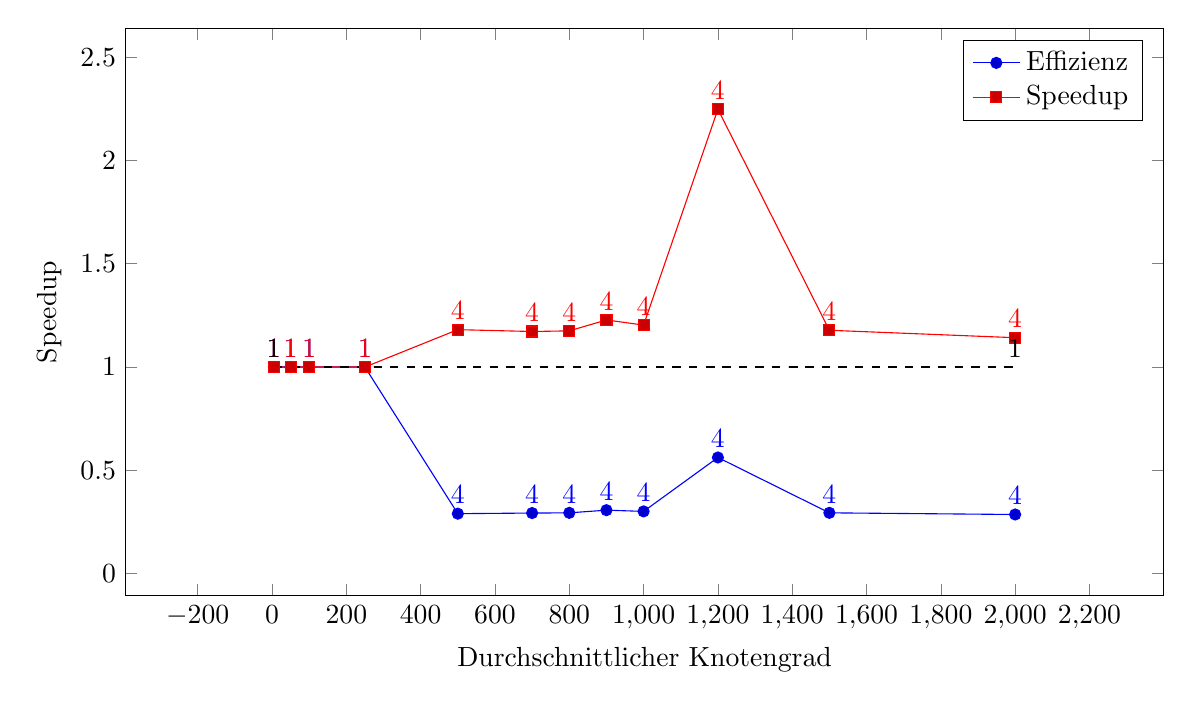
\begin{tikzpicture}
		\begin{axis}[nodes near coords,
			enlargelimits=0.2,
			width=420, height=250,
			xlabel=Durchschnittlicher Knotengrad,
	        ylabel=Speedup]

		    \addplot+[	        
		        point meta=explicit symbolic]
		    coordinates {
		        (5,1) [1]
		        (50,1) [1]
		        (100,1) [1]
		        (250,1) [1]
		        (500,0.29) [4]
		        (700,0.293) [4]
		        (800,0.294) [4]
		        (900,0.307) [4]
		        (1000,0.301) [4]
		        (1200,0.562) [4]
		        (1500,0.294) [4]
		        (2000,0.286) [4]
		    };
		    \addlegendentry{Effizienz}

		    \addplot+[
		        point meta=explicit symbolic]
		    coordinates {
		        (5,1) [1]
		        (50,1) [1]
		        (100,1) [1]
		        (250,1) [1]
		        (500,1.181) [4]
		        (700,1.172) [4]
		        (800,1.175) [4]
		        (900,1.228) [4]
			    (1000,1.203) [4]
			    (1200,2.248) [4]
			    (1500,1.178) [4]
			    (2000,1.142) [4]
			};
		    \addlegendentry{Speedup}

		    \addplot+[
		        smooth,
		        dashed,
		        black,
		        mark=none]
		    coordinates {
		    	(5,1)
		    	(2000,1)
		    };

		\end{axis}
	\end{tikzpicture}
\end{figure}

\begin{figure}
	\centering
	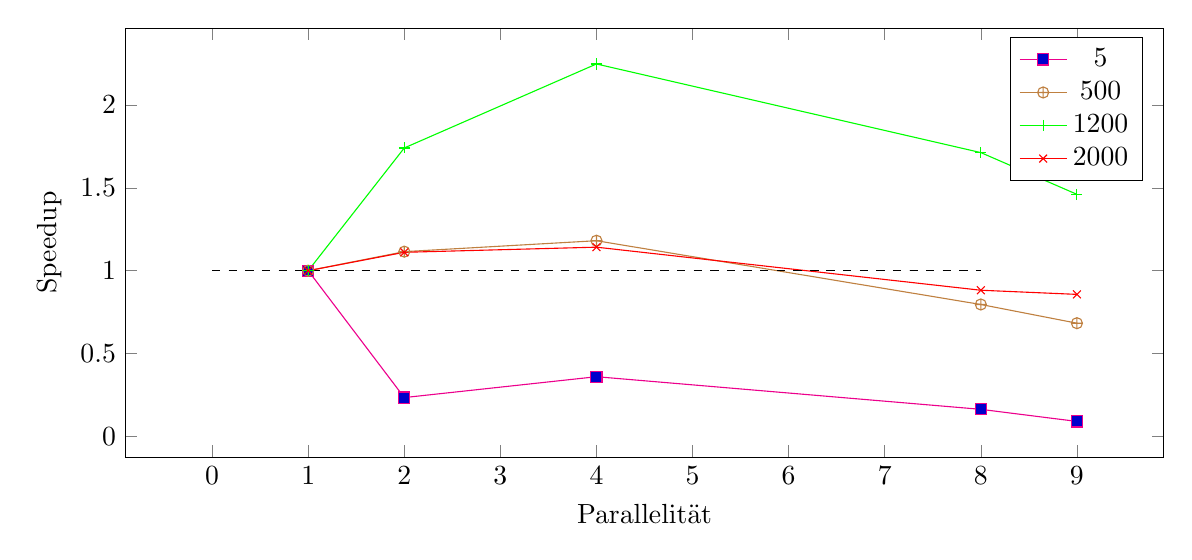
\begin{tikzpicture}
		\begin{axis}[
	        xlabel=Parallelität,
	        ylabel=Speedup,
	        width=420, height=200]

		    \addplot+[
		    magenta,
		    solid,
		    mark=square*]
		    coordinates {
		        (1,1)
		        (2,0.234)
		        (4,0.36)
		        (8,0.163)
		        (9,0.090)
		    };
		    \addlegendentry{5}

		    \addplot+[
		    brown,
		    solid,
		    mark=oplus]
		    coordinates {
		        (1,1)
		        (2,1.115)
		        (4,1.181)
		        (8,0.796)
		        (9,0.683)
		    };
		    \addlegendentry{500}

		    \addplot+[
		    green,
		    solid,
		    mark=+]
		    coordinates {
		        (1,1)
		        (2,1.741)
		        (4,2.248)
		        (8,1.713)
		        (9,1.461)
		    };
		    \addlegendentry{1200}

		    \addplot+[
		    red,
		    solid,
		    mark=x]
		    coordinates {
		        (1,1)
		        (2,1.111)
		        (4,1.142)
		        (8,0.882)
		        (9,0.857)
		    };
		    \addlegendentry{2000}

		    \addplot+[
		        smooth,
		        dashed,
		        black,
		        mark=none]
		    coordinates {
		    	(0,1)
		    	(8,1)
		    };

		\end{axis}
	\end{tikzpicture}
	\caption{Speedup des 1D-Algorithmus über Anzahl der Places. Die Dichte variiert. Als Referenzwert wurde jeweils der schnellste serielle Algorithmus genommen. Es wurden immer die schnellsten, gemessenen Werte verwendet.}
	\label{fig:verteilung_dichte}
\end{figure}
% subsection dichte (end)
%!TEX root = thesis.tex
\subsection{Verteilung} % (fold)
\label{sub:verteilung}
Die Ergebnisse der hier besprochen Testreihe, finden sich allesamt in Anhang \ref{Anhang-Messwerte-Verteilung}. Bei der Testreihe wurde die Knotenzahl fest auf 100 000 festgelegt und der durchschnittliche Kantengrad fest auf 750 eingestellt. Jeder Graph hat also auch die selbe absolute Kantenzahl. Diese Zahl wurde relativ hoch angesetzt, um genug Spielraum für die Variation der Verteilung zu haben. Ein Graph, dessen minimaler und maximaler Knotengrad weit vom durchschnittlichen Knotengrad entfernt ist, wird \textit{ungleichmäßig} genannt. Das Gegenteil dazu wird als \textit{gleichmäßig} bezeichnet. 

Zunächst fällt auf, dass die seriellen Laufzeiten in der Praxis konstant sind, wie es die Theorie vorhersagt. Dadurch ist in dieser Testreihe der Speedup besonders gut vergleichbar. In Abbildung \ref{fig:verteilung_speedup} ist die oberste Kurve der Speedup des gleichmäßigsten Graphen und die untere Kurve die, des ungleichmäßigsten Graphen. Es ist deutlich ersichtlich, dass das Parallelisierungspotential eines Graphen stark von der Verteilung der Knotengrade abhängt. Um so gleichmäßiger diese verteilt sind, um so besser funktioniert die Parallelisierung. Ein mögliche Erklärung ist, dass bei einem gleichmäßig verteilten Graph die Wahrscheinlichkeit größer ist, dass die Rechenlast gleichmäßig auf alle Places verteilt wird. Bei ungleichmäßigen Graphen hingegen, ist es eher zufällig, auf welchem Place wie viele aktive Knoten liegen. Auf die Größe der Datenmengen, die zwischen den Places transportiert werden muss, dürfte die Verteilung keinen Einfluss haben.

\begin{figure}
	\centering
	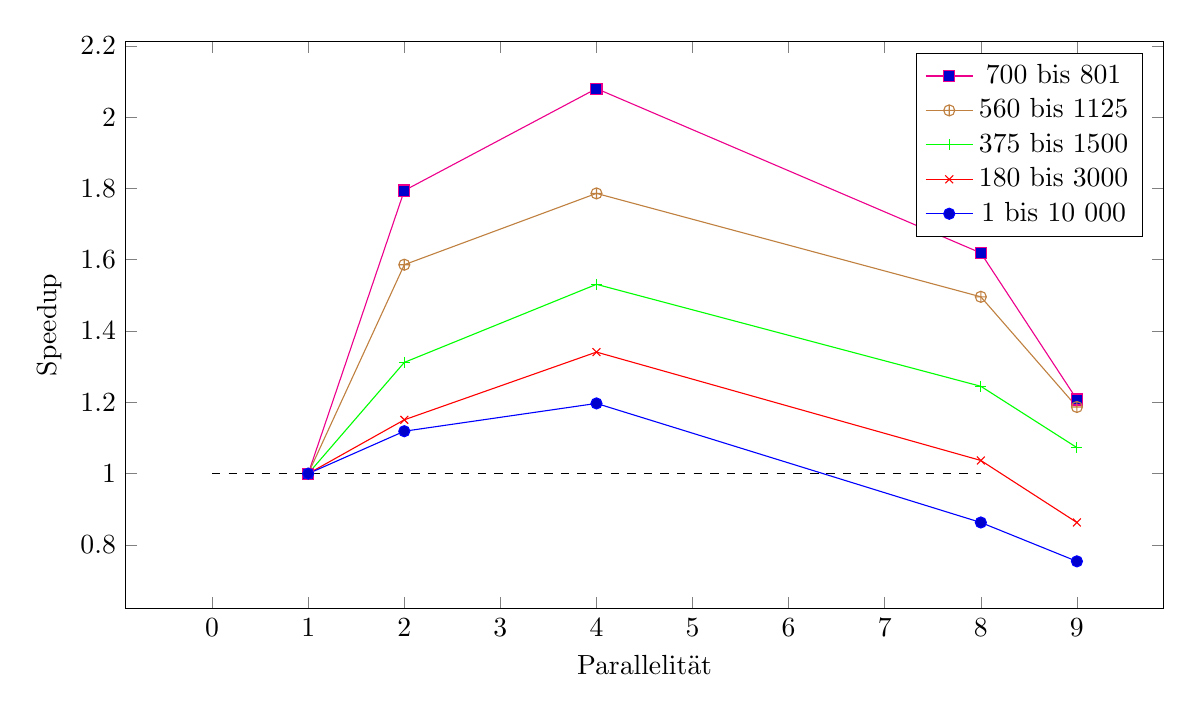
\begin{tikzpicture}
		\begin{axis}[
	        xlabel=Parallelität,
	        ylabel=Speedup,
	        width=420, height=250]

		    \addplot+[
		    magenta,
		    solid,
		    mark=square*]
		    coordinates {
		        (1,1)
		        (2,1.794)
		        (4,2.080)
		        (8,1.619)
		        (9,1.208)
		    };

		    \addlegendentry{700 bis 801}
		    \addplot+[
		    brown,
		    solid,
		    mark=oplus]
		    coordinates {
		        (1,1)
		        (2,1.586)
		        (4,1.786)
		        (8,1.496)
		        (9,1.187)
		    };
		    \addlegendentry{560 bis 1125}

		    \addplot+[
		    green,
		    solid,
		    mark=+]
		    coordinates {
		        (1,1)
		        (2,1.312)
		        (4,1.531)
		        (8,1.245)
		        (9,1.073)
		    };
		    \addlegendentry{375 bis 1500}

		    \addplot+[
		    red,
		    solid,
		    mark=x]
		    coordinates {
		        (1,1)
		        (2,1.151)
		        (4,1.341)
		        (8,1.037)
		        (9,0.863)
		    };
		    \addlegendentry{180 bis 3000}

		    \addplot+[
		    blue,
		    solid,
		    mark=*]
		    coordinates {
		        (1,1)
		        (2,1.119)
		        (4,1.197)
		        (8,0.863)
		        (9,0.754)
		    };
		    \addlegendentry{1 bis 10 000}

		    \addplot+[
		        smooth,
		        dashed,
		        black,
		        mark=none]
		    coordinates {
		    	(0,1)
		    	(8,1)
		    };

		\end{axis}
	\end{tikzpicture}
	\caption{Speedup des 1D-Algorithmus über Anzahl der Places. Die Verteilung variiert. Als Referenzwert wurde jeweils der schnellste serielle Algorithmus genommen. Pro Graph ist eine Kurve eingezeichnet. Es wurden immer die schnellsten, gemessenen Werte verwendet.}
	\label{fig:verteilung_speedup}

\end{figure}
% subsection verteilung (end)
%!TEX root = thesis.tex
\subsection{Größe} % (fold)
\label{sub:gr_e}
Die Testreihe, um die Auswirkung der Größe eines Graphen auf die Algorithmen herauszufinden, orientiert sich an einem Socialgraph. Es wurde geschätz, dass jeder durchschnittlich 100 Freunde hat, jeder mehr als einen Freund hat und keiner mehr als 500 Freunde hat. Das ergibt einen durchschnittlichen Knotengrad von 100, wobei der Knotengrad zwischen 1 und 500 liegt. Variiert wurde nun die Größe der Graphen. Es handelt sich hier um relativ dünn besetzte Graphen, so dass selbst der 500 000 Knoten Graph noch unter 500 MB liegt. Es wurde versucht, die Graphgröße weiter auf bis zu 2 Millionen Knoten zu steigern, was allerdings nicht möglich war. Graphen mit vielen Knoten resultieren in großen Sendepuffern und wie sich herausstellte, ist X10 dem nicht gewachsen. Der Sendevorgang (der \textit{at} Block) wird in den meisten fällen nie verlassen. Deswegen wurde hier die Knotenzahl auf 500 000 beschränkt. Es ist zu vermuten, dass diese Größe nicht ausreicht, um gute Ergebnisse bei der Parallelisierung zu erreichen.

Des weiteren wurde in dieser Testreihe der Modus mit 9 Places und der invasive Algorithmus weggelassen. Dass mit 9 Places auf 8 Kernen die Performance nicht gut sein wird, war bereits zu erwarten und bestätigte sich. Der invasive Algorithmus hatte ebenso Probleme mit der Graphgröße, was zwar durch Implementierungstricks umgangen werden könnte, aber allerdings den Zeitrahmen gesprengt hätte. Wieso der invasive Algorithmus nicht funktioniert, ist in der Bemerkung unten erläutert.

Bei jedem Graph dieser Testreihe war die serielle Version am schnellsten, was nach den vorangegangenen Ergebnissen auf keinen Fall zu erwarten war. Die serielle Version war schneller als jeder andere Algorithmus, egal mit wie vielen Places. Im Kapitel \ref{sub:dichte}, in dem die Dichte variierte, war der 1D-Algorithmus schon im Fall mit nur einem Place schneller, als der serielle Algorithmus. Da das hier nicht auftritt, ist zu vermuten, dass der 1D Algorithmus für dichte Graphen ein wenig schneller zu sein scheint, während der serielle Algorithmus für dünn besetzte Graphen schneller ist.
% TODO: Begründung? 

Vergleicht man nur den 1D-Algorithmus mit sich selbst bei steigender Anzahl an Places, zeichnet sich das Bild, dass 2 Places das Maximum zu sein scheint. In Abbilgun \ref{fig:groesse_speedup} ist sehr schön zu sehen, dass der Algorithmus mit 2 Places immer schneller war, als der Algorithmus mit 4 Places. Bei 8 Places war der Speedup immer kleiner als 1, was langsamere Laufzeit als die Referenzzeit bedeutet. Wie zu erwarten steigt tendenziell mit der Anzahl der Knoten das Parallelisierungspotential, wobei es durch den dünn besetzte Graph einigermaßen beschränkt zu sein scheint. Wäre dem nicht so müsste der Algorithmus auf 4 Places gegenüber den 2 Places aufholen, bei steigender Knotenzahl.

Für den 2D Algorithmus gilt, dass nie ein Speedup kleiner 1 erreicht wurde. Die hier verwendeten Graphen sind dafür zu klein.

\begin{figure}
	\centering
	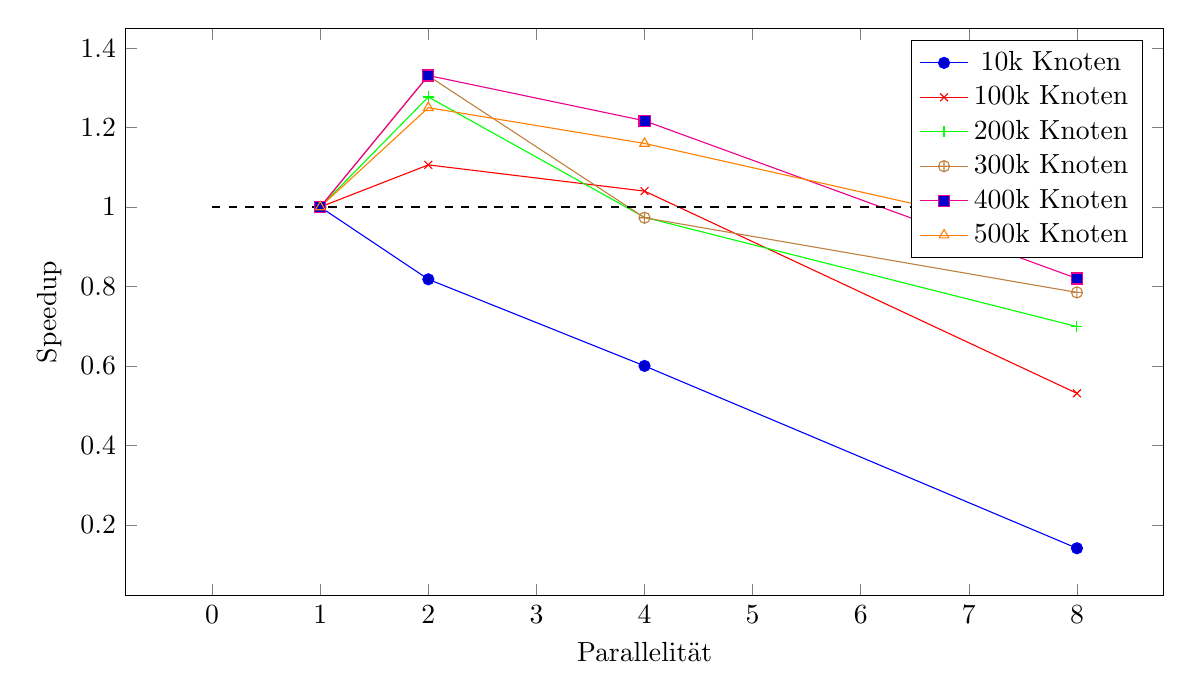
\begin{tikzpicture}
		\begin{axis}[
	        xlabel=Parallelität,
	        ylabel=Speedup,
	        width=420, height=250]

		    \addplot+[
		    blue,
		    solid,
		    mark=*]
		    coordinates {
		        (1,1)
		        (2,0.818)
		        (4,0.6)
		        (8,0.141)
		    };
		    \addlegendentry{10k Knoten}

		    \addplot+[
		    red,
		    solid,
		    mark=x]
		    coordinates {
		        (1,1)
		        (2,1.106)
		        (4,1.04)
		        (8,0.531)
		    };
		    \addlegendentry{100k Knoten}

		    \addplot+[
		    green,
		    solid,
		    mark=+]
		    coordinates {
		        (1,1)
		        (2,1.277)
		        (4,0.974)
		        (8,0.699)
		    };
		    \addlegendentry{200k Knoten}

		    \addplot+[
		    brown,
		    solid,
		    mark=oplus]
		    coordinates {
		        (1,1)
		        (2,1.330)
		        (4,0.973)
		        (8,0.785)
		    };
		    \addlegendentry{300k Knoten}

		    \addplot+[
		    magenta,
		    solid,
		    mark=square*]
		    coordinates {
		        (1,1)
		        (2,1.331)
		        (4,1.217)
		        (8,0.82)
		    };
		    \addlegendentry{400k Knoten}

		    \addplot+[
		    orange,
		    solid,
		    mark=triangle]
		    coordinates {
		        (1,1)
		        (2,1.25)
		        (4,1.16)
		        (8,0.916)
		    };
		    \addlegendentry{500k Knoten}

		    \addplot+[
		        smooth,
		        dashed,
		        black,
		        mark=none]
		    coordinates {
		    	(0,1)
		    	(8,1)
		    };

		\end{axis}
	\end{tikzpicture}
	\caption{Speedup des 1D-Algorithmus über Anzahl der Places. Variiert wurde die Größe des Graphen. Als Referenzwert wurde jeweils der 1D-Algorithmus mit einem Place genommen. Eine Kurve pro Graph.}
	\label{fig:groesse_speedup}
\end{figure}

\underline{Bemerkung:}
Beim Parsen der Graphdatei gehen alle Implementierungen so vor, dass sie Zeile für Zeile in die Datenstruktur eingepflegt werden. Dabei steht schon vor dem Parsen fest, welches Datum auf welchen Place muss. Die Informationshäppchen, die von Place zu Place übertragen werden müssen, sind relativ klein. Im invasiven Fall ergibt es wenig Sinn, schon ein \textit{invade} aufzurufen, bevor überhaupt der Graph eingelesen wurde, bevor also die Größe des Problems bekannt ist. Aus diesem Grund wird der Graph erst lokal auf den ersten Place eingelesen, dann der Constraint zusammengebaut und erst wenn der Claim bekannt ist, auf die involvierten Places verteilt. Die hier zu übetragenen Daten sind relativ groß, womit X10 Probleme zu haben scheint. Das Problem könnte umgangen werden, indem die Datenstruktur in kleinere Häppchen aufgeteilt wird. Das ist aber höchstens ein Workaround um ein Problem, das bei X10 liegt.
% subsection gr_e (end)

% section ergebnisse_der_parallelisierung (end)

\section{Die 2D Breitensuche} % (fold)
\label{sec:die_2d_breitensuche}
Die 2D Breitensuche ist in jedem Testfall der mit Abstand langsamste Algorithmus gewesen, was so nicht zu erwarten war. Der implementierte Algorithmus ist zwar zunächst deutlich komplexer, als die anderen beiden, doch gibt es zwei theoretische Vorteile, die diesen Algorithmus studierenswert machen. Erstens sind die Gruppen von Places, die untereinander kommunizieren deutlich kleiner. In der ersten Kommunikationsphase sendet jeder Place seine Daten an eine ganze Spalte, und empfängt dafür von einer ganzen Zeile die Daten für den nächsten Schritt. Das sind $2 * \sqrt(p)$ Places, insgesamt, mit denen jeder Place kommunizieren muss, also $O(p * 2 + \sqrt(p) * \frac{1}{2}) = O(p * \sqrt(p))= O(p^{\frac{3}{2}})$ Kommunikationsvorgänge im System. In der zweiten Kommunikationsphase muss jeweils nur eine Zeile miteinander kommunizieren. Das sind zusätzlich $O(\sqrt(p) * p * \frac{1}{2})$ Kommunikationsvorgänge. Es sind also im O-Kalkül pro Iteration $O(p^{\frac{3}{2}})$. Im Vergleich dazu kommuniziert jeder Place im 1D Algorithmus mit allen anderen p-1 Places, also $O(p^2)$ Kommunikationsvorgänge. Der zweite Vorteil der Implementierung wie in \cite{Buluc:2011} ist die Möglichkeit, alle Kommunikation und Synchronisation auf drei MPI Operationen abzubilden. Die auf entsprechender Hardware vergleichsweise schnell sind. 

Beide dieser Vorteile sind bei der X10 Implementierung, die auf nur einem CPU läuft, hinfällig. Zunächst wurden die MPI Operationen in X10 \enquote{nachprogrammiert}. Um das zu tun, muss \textit{at} verwendet werden, dass einen für diesen Zweck unnützen Rückkanal bereithält, der zusätzliche Latenz in jede Kommunikation bringt. Weiterhin gibt es bei der Verwendung einer hochperformanten MPI Hardware den Vorteil, dass ein Datum nur einmal gesendet werden muss, wenn es an mehrere Empfänger gehen soll. Das ist in X10-Syntax nicht möglich. Die zusätzliche Kommunikation ist also teurer, als sie sein müsste. 
Der zweite Vorteil, eben dass weniger Kommunikationsvorgänge im System sind, ist aus zwei Gründen hier nicht ausschlaggebend. Zum einen sind dermaßen wenig Places im Spiel, dass es kaum einen Unterschied zwischen $O(p^{\frac{3}{2}})$ und $O(p^2)$ gibt, zum anderen haben erste Tests gezeigt, dass die Kommunikationsphasen etwa 4 bis 5 Mal so schnell sind wie die Rechenphasen, also die Kommunikation nicht so ausschlaggebend ist, wie das zu erwarten war. Das wiederum ist auf die Testumgebung ohne wirklich getrennte Places zurückzuführen.

Wie in \cite{Buluc:2011} ist also auch in X10 die 2D Implementierung eher die schlechtere, wobei in den Dimensionen, in denen in dieser Arbeit gedacht wird, die Unterschiede gravierender sind. Ob in größeren Testumgebungen die Ergebnisse anders ausfallen, muss in einer weiteren Arbeit untersucht werden.
% section die_2d_breitensuche (end)

\section{Invasive Breitensuche} % (fold)
\label{sec:invasive_breitensuche}
Im Rahmen dieser Arbeit wurden Ansätze herausgearbeitet, um die Breitensuche an das invasive Rechnen im Allgemeinen und an das Framework invadeX10 im Speziellen, anzupassen. Als Grundlage diente dazu der 1D-Algorithmus. Die invasive Version ist prinzipiell der selbe Algorithmus. Die zusätzliche Funktionalität und die zusätzlichen Schwierigkeiten, die in Kapitel \ref{sec:unterschiede_zum_nicht_invasiven_fall} beschrieben sind, generieren aber pro Iteration viel Overhead. Dadurch, dass der Kontrollfluss nach jeder Iteration wieder zur Masteractivity zurückkehrt, ist auch zusätzliche Kommunikationsaufwand notwendig. Die gemessenen Laufzeiten sind erwartungsgemäß  langsamer, als die der 1D-Breitensuche und aus den eben genannten Gründen nicht vergleichbar. Allgemein ist es unfair und vor allem nicht zielführend, die benötigte Zeit zur Lösung einer einzelnen BFS-Instanz zu vergleichen, da im invasiven Rechnen bewusst Nachteile bei der Lösung einer einzelnen Instanz in Kauf genommen werden, um eine Menge von Rechenjobs als Ganzes schneller bewältigt zu können. Die Intention des invasiven Rechnens ist nicht, eine einzelne Instanz möglichst schnell zu lösen. Um einen fairen Vergleich durchzuführen, muss eine Menge von verschiedenen Jobs und eine Zielhardware definiert werden. Daraufhin muss verglichen werden, wie lange es mit verschiedenen Strategien braucht, bis alle Jobs erledigt wurden. Die Strategien sind zum Beispiel, alle gleichzeitig starten, ein Job nach dem anderen starten oder eben invasives Vorgehen. In Mangel der invasiven Hardware und ausgereiften Softwareinstrumenten um diese zu simulieren, musste darauf in dieser Arbeit verzichtet werden. Die Ergebnisse sind aber insofern nicht schlecht, als dass die invasive Breitensuche in den Testläufen besser mit der Anzahl der Places skalierte, als die 2D-Breitensuche.  Für das beschriebene Testsetup ist der vorliegende Algorithmus somit ein guter Ausgangspunkt.
% section invasive_breitensuche (end)


% section wikipedia_und_die_philosopie (end)
% chapter ergebnisse_und_diskussion (end)
%!TEX root = thesis.tex
\chapter{Fazit und zukünftige Arbeit} % (fold)
\label{cha:fazit_und_zuk_nftige_arbeit}
\underline{\textbf{Fazit:}}
In dieser Arbeit wurden zwei Strategien, die Breitensuche zu Parallelisieren, auf die moderne Programmiersprache X10 übertragen und getestet. Dazu wurde in mehreren Iterationen durch Tests und Veränderungen am Code, der Algorithmus so weit wie möglich optimiert und an die Parallelitätskonstrukte von X10 angepasst. Eine der beiden Strategien, die 1D-Breitensuche wurde zusätzliche für das invasive Framework invadeX10 angepasst. Dabei wurde besonders auf die dabei neu auftretenden Probleme und deren Lösungen eingegangen, sowie erwähnt, an welchen Stellen noch zusätzliche Arbeit notwendig ist.

Die Messungen ergaben, dass sich die 1D-Dekomposition im kleinen Maßstab wesentlich besser eignet, als die 2D-Dekomposition, deren zusätzliche Komplexität sich nicht auszahlt. Ob überhaupt eine Parallelisierung sinnvoll ist, hing dabei stark von dem gewählten Graph ab. Es scheint, als bräuchte man eine mindeste Anzahl von Knoten und einen möglichst gleichverteilten Knotengrad, um gute Ergebnisse zu erhalten. Die verwendete Hardware in Verbindung mit den verwendete Messmethoden lassen eine Übertragbarkeit der Ergebnisse auf Rechencluster aber nicht zu. Ebenso sind die Ergebnisse für Shared-Memory Systeme kaum aussagekräftig. Die Algorithmen sind nur ein Zwischenschritt auf dem Weg zum invasiven Rechnen oder den Manycore-Systemen der Zukunft.
\newline\newline
\underline{\textbf{Zukünftige Arbeit:}}
Im Rahmen dieser Arbeit konnten einige Ideen und Ansätze nicht umgesetzt werden, die in zukünftiger Arbeit anzugehen sind.

Um die bestehende Arbeit besser zu testen und um die Vor- und Nachteile besser zu verstehen, sollte der existierende Code auf einem echten Rechencluster getestet werden. Die Bedingungen unterscheiden sich stark von der parallelen Ausführung auf nur einem Prozessor. Zum einen können mit einem Rechencluster, das echten verteilten Speicher hat, wesentlich größere Graphen getestet werden. Größere Graphen bedeuten immer auch, das ein größeres Parallelisierungspotential vorhanden sein kann. Zum anderen ist X10 laut den Entwicklern dafür gemacht, effiziente Programme für große verteilte Rechensysteme zu programmieren. Aus diesen zwei Gründen ist zu erwarten, dass der in dieser Arbeit erreichte Speedup weit unter dem Potential der Breitensuche geblieben ist. 

Zudem muss die Breitensuche natürlich auf der Invasiven Hardware getestet werden, die im Rahmen des invasIC Projekts entsteht.

Auch implementierungstechnisch gibt es weitere Variationsmöglichkeiten, deren Auswirkung auf Geschwindigkeit und Beschleunigung getestet werden kann. Die einzelnen Processing Elements können auch autonomer Implementiert werden, als sie es im Moment sind. Wenn jede PE ein eigenes Intervall des Graphen bekommt und darauf autonom rechnet, würde die Synchronisation zwischen den einzelnen PEs komplett wegfallen. In der aktuellen Codebasis wäre das eine Barriere weniger. Außerdem sparte man sich die Funktionsaufrufe und die Arithmetik, um die Liste der aktiven Knoten aufzuteilen. Der Nachteil dieser Implementierung wäre, dass von einem Place zu einem anderen pro Iteration mehrere Kommunikationen stattfinden, falls mehrere PEs zum gleichen Place senden müssen. 

In der invasiven Implementierung werden im Moment keine Processing Elements abgegeben oder neu beantragt, sobald der Algorithmus einmal gestartet ist. Die Masteractivity weiß aber nach jeder Iteration, wie lang die Liste der aktiven Knoten auf jedem Place ist. Mit dieser Information könnte sie Rechenleistung freigeben oder neu beantragen. Eine entsprechende Implementierung würde die Möglichkeit des Framework nutzen, eine einmal abgegebene PE wieder zurück zu verlangen. Diese Funktion würde das in Kapitel \ref{sub:dynamische_ressourcenverwaltung} beschriebenen Problem lösen, dass anzunehmender Weise zu einem späteren Zeitpunkt genau die abgegebene Rechenleistung wieder gebraucht wird. Diese Funktionalität ist aber noch nicht vorhanden und konnte somit nicht getestet werden. 

Darüber hinaus wurde nicht getestet, wie sich ein Programm verhält, wenn die Datenhaltung auf eine veränderte Situation der Rechenleitung reagiert. Dieser Ansatz geht im Gegensatz zu dem gerade genannten davon aus, dass Rechenleistung genutzt werden soll, egal auf welchem Place sie liegt. Wenn also Rechenleistung abgegeben wurde oder neue hinzukam, müssen die Graphdaten dynamisch entsprechend an den richtigen Ort kopiert werden. Womöglich können die Daten so verteilt werden, dass ab einem gewissen Zeitpunkt für jeden Knoten mindestens zwei Places verantwortlich sind und dadurch auf weitere Änderungen sehr schnell reagiert werden kann.

Zu guter Letzt muss der invasive Algorithmus wie in Kapitel \ref{sec:invasive_breitensuche} beschrieben in einem Setup getestet werden, in dem viele Instanzen gleichzeitig gelöst werden sollen, um die Vorteile des invasiven Rechnens überhaupt nutzen zu können.


% chapter fazit_und_zuk_nftige_arbeit (end)


%% --------------------
%% |   Bibliography   |
%% --------------------
\cleardoublepage
\nocite{*}
\phantomsection
\addcontentsline{toc}{chapter}{\bibname}

\iflanguage{english}
{\bibliographystyle{IEEEtranSA}}	% english style
{\bibliographystyle{babalpha-fl}}	% german style
												  
% Use IEEEtran for numeric references
%\bibliographystyle{IEEEtranSA})

\bibliography{thesis}


%% ----------------
%% |   Appendix   |
%% ----------------
\cleardoublepage

%!TEX root = thesis.tex
%%

%% ==============================
%\chapter{Appendix}
%\label{ch:Appendix}
%% ==============================

\appendix
\addchap{Anhang}

\section{Messwerte - Dichte}
\label{Anhang-Messwerte-Dichte}
Alle Messwerte sind in Millisekunden (ms) angegeben. Alle Graphen haben 100 000 Knoten. Der Name \nobreak{avX} steht für einen Graphen mit 100 000 Knoten und einem durchschnittlichen Ausgangsgrad von X. Alle Algorithmen verwenden Arraylisten als Datenstruktur. Der invasive Algorithmus wurde mit einem PE pro Place ausgeführt. Zwischen den Iterationen wurde nichts an dem Claim geändert. Der Knotengrad liegt bei allen Algorithmen zwischen 1 und $\infty$.
%!TEX root = thesis.tex
\begin{center}
\csvautotabular{Laufzeiten/Dichte/100kav5.csv} \\ \vspace{1cm}
\csvautotabular{Laufzeiten/Dichte/100kav50.csv} \\ \vspace{1cm}
\csvautotabular{Laufzeiten/Dichte/100kav100.csv} \\ \vspace{1cm}
\csvautotabular{Laufzeiten/Dichte/100kav250.csv} \\ \vspace{1cm}
\csvautotabular{Laufzeiten/Dichte/100kav500.csv} \\ \vspace{1cm}
\csvautotabular{Laufzeiten/Dichte/100kav700.csv} \\ \vspace{1cm}
\csvautotabular{Laufzeiten/Dichte/100kav800.csv} \\ \vspace{1cm}
\csvautotabular{Laufzeiten/Dichte/100kav900.csv} \\ \vspace{1cm}
\csvautotabular{Laufzeiten/Dichte/100kav1000.csv} \\ \vspace{1cm}
\csvautotabular{Laufzeiten/Dichte/100kav1200.csv} \\ \vspace{1cm}
\csvautotabular{Laufzeiten/Dichte/100kav1500.csv} \\ \vspace{1cm}
\csvautotabular{Laufzeiten/Dichte/100kav2000.csv} \\ \vspace{1cm}
\end{center}
 

\clearpage
\section{Messwerte - Verteilung}
\label{Anhang-Messwerte-Verteilung}
Alle Messwerte sind in Millisekunden (ms) angegeben. Jeder Graph hat 100 000 Knoten und einen durchschnittlichen Knotengrad von 750. Der invasive Algorithmus wurde mit einem PE pro Place ausgeführt. Zwischen den Iterationen wurde nichts an dem Claim geändert.
\begin{center}
\csvautotabular{Laufzeiten/Verteilung/av750_1_10000.sgraph.csv} \\ \vspace{1cm}
\csvautotabular{Laufzeiten/Verteilung/av750_180_3000.sgraph.csv} \\ \vspace{1cm}
\csvautotabular{Laufzeiten/Verteilung/av750_375_1500.sgraph.csv} \\ \vspace{1cm}
\csvautotabular{Laufzeiten/Verteilung/av750_560_1125.sgraph.csv} \\ \vspace{1cm}
\csvautotabular{Laufzeiten/Verteilung/av750_700_801.sgraph.csv} \\ \vspace{1cm}
\end{center}

\clearpage
\section{Messwerte - Größe}
\label{Anhang-Messwerte-Groesse}
Alle Messwerte sind in Millisekunden (ms) angegeben. Jeder Graph hat einen durchschnittlichen Knotengrad von 100, wobei der Knotengrad jedes Knotens zwischen 1 und 500 liegt. Es wurde auf den invasiven Algorithmus verzichtet, da die Hardware größeren Graphen mit diesem Algorithmus nicht gewachsen ist. Auf die Testläuft mit 9 Places wurde ebenso verzichtet.
%!TEX root = thesis.tex
\begin{figure}[h]
\begin{minipage}[t]{8cm} 
\begin{center} 
\tiny\csvautotabular{Laufzeiten/groesse/10k.sgraph.csv}
\end{center} 
\end{minipage} 
\hfill 
\begin{minipage}[t]{7.5cm}
\begin{center} 
\tiny\csvautotabular{Laufzeiten/groesse/100k.sgraph.csv}
\end{center} 
\end{minipage} 
\end{figure}

\begin{figure}[h]
\begin{minipage}[t]{8cm} 
\begin{center} 
\tiny\csvautotabular{Laufzeiten/groesse/200k.sgraph.csv}
\end{center} 
\end{minipage} 
\hfill 
\begin{minipage}[t]{7.5cm}
\begin{center} 
\tiny\csvautotabular{Laufzeiten/groesse/300k.sgraph.csv}
\end{center} 
\end{minipage} 
\end{figure}

\begin{figure}[h] 
\begin{minipage}[t]{8cm} 
\begin{center} 
\tiny\csvautotabular{Laufzeiten/groesse/400k.sgraph.csv}
\end{center} 
\end{minipage} 
\hfill 
\begin{minipage}[t]{7.5cm}
\begin{center} 
\tiny\csvautotabular{Laufzeiten/groesse/500k.sgraph.csv}
\end{center} 
\end{minipage} 
\end{figure}

% \setcounter{figure}{0}
		
% \begin{figure} [ht]
%   \centering
%    ein Bild
%   \caption{A figure}
%   \label{fig:BPMNBeispiela}
% \end{figure}


\end{document}
